% ===========================================================================
%  stab0 — 格点QCD胶子PDF蒸馏计算管线对照分析报告
%  Comparative Analysis of GPU Distillation Pipelines:
%  docker-v20260803 / docker-v20260804 / docker-v20260805
%  Zhang Xin (IMP, CAS)  2026-08-03
% ===========================================================================
\documentclass[11pt,a4paper]{article}

% ── 中文支持 ──
\usepackage[UTF8]{ctex}
\setCJKmainfont{AR PL SungtiL GB}[BoldFont=AR PL UMing CN]
\setCJKsansfont{AR PL KaitiM GB}[BoldFont=AR PL UMing CN]
\setCJKmonofont{AR PL UMing CN}

% ── 数学 ──
\usepackage{amsmath,amssymb,amsfonts}
\usepackage{physics}
\usepackage{braket}
\usepackage{bm}

% ── 排版 ──
\usepackage[margin=2.5cm]{geometry}
\usepackage{booktabs}
\usepackage{graphicx}
\usepackage[colorlinks=true,linkcolor=blue,citecolor=blue,urlcolor=blue]{hyperref}
\usepackage{enumitem}
\usepackage{caption}
\usepackage{subcaption}
\usepackage{multirow}
\usepackage{array}
\usepackage{float}
\usepackage{siunitx}

% ── 自定义命令 ──
\newcommand{\gev}{\;\mathrm{GeV}}
\newcommand{\fm}{\;\mathrm{fm}}
\newcommand{\fmto}{\;\mathrm{fm}^{-1}}
\newcommand{\conf}{\mathrm{config}}
\newcommand{\meff}{m_{\mathrm{eff}}}
\newcommand{\Nconf}{N_{\mathrm{conf}}}
\newcommand{\Nev}{N_{\mathrm{ev}}}
\newcommand{\Nt}{N_t}
\newcommand{\Nx}{N_x}
\newcommand{\tsep}{t_{\mathrm{sep}}}
\newcommand{\tsrc}{t_{\mathrm{src}}}
\newcommand{\tsink}{t_{\mathrm{sink}}}
\newcommand{\Ctwo}{C^{(2)}}
\newcommand{\CtwoI}{C^{(2),I}}
\newcommand{\CtwoF}{C^{(2),F}}
\newcommand{\Cthree}{C^{(3)}}
\newcommand{\Em}{E^{(0)}}
\newcommand{\EmP}{E^{(0)}(p_z)}
\newcommand{\pmom}{p_z}
\newcommand{\apm}{a^{-1}}
\newcommand{\jack}{\mathrm{JK}}
\newcommand{\gmu}{\gamma_\mu}
\newcommand{\vi}{\vec{v}^{\,(k)}}
\newcommand{\mone}{M^{-1}}

\title{\textbf{格点QCD胶子PDF蒸馏计算管线对照分析报告}\\[0.4em]
       \large docker-v20260803 \ \texttt{vs.}\ docker-v20260804 \ \texttt{vs.}\ docker-v20260805\\[0.3em]
       （以 docker-v20260805 为范例）}
\author{张鑫\thanks{中国科学院近代物理研究所 (IMP, CAS)}}
\date{2026年8月3日}

\begin{document}
\maketitle

\begin{abstract}
本报告对三条基于蒸馏(Distillation)方法、在GPU(CUDA/CuPy)上实现的格点QCD胶子PDF验证管线
——\texttt{docker-v20260803}、\texttt{docker-v20260804} 与 \texttt{docker-v20260805}——
进行完整的数据、图表与理论物理对照分析。三者共用同一CLQCD组态集合
($\beta=6.20$, $24^3\times72$, $a\approx0.1053\;\fm$, $\apm\approx1.874\;\gev$,
$m_\pi\approx300\;\mathrm{MeV}$)，但在组态数、本征矢数、关联函数集、OPE算符与统计分析上逐级演进。
以功能最完整的 \texttt{docker-v20260805}（10组态、$\Nev=100$、自包含 \texttt{lib/}、含胶子OPE与
三点/四点关联函数）为范例展开。主要物理结果：$\pi$介子静止质量 $m_\pi=0.286(2)\;\gev$，
质子质量 $m_p=1.118(8)\;\gev$（高于物理值约$19\%$，符合该系综较重夸克质量的预期），
色散关系在 $P_z=2$ 处符合良好；质子--中子两点函数因味守恒恒为零；donghx胶子OPE算符与
v20260802 完全一致（相关系数$=1.0$）。对照分析指出三版本在统计精度、动量道质量与
分析深度上的关键差异与改进路径。
\end{abstract}

\tableofcontents
\newpage

% ===========================================================================
\section{引言}
% ===========================================================================
核子（质子）中的非极化胶子部分子分布函数(PDF) $g(x,\mu)$ 是理解质子自旋与质量结构、
以及在大型强子对撞机上刻画初始态胶子密度的核心量。格点QCD原则上可从第一原理计算PDF，
但PDF定义为光锥上算符的矩阵元，在欧几里得格点上无法直接计算。

\textbf{大动量有效理论(LaMET)}~\cite{ji2013,ji2021} 提供了一条可行路径：计算强子在大动量
$p_z\gg \Lambda_{\mathrm{QCD}}$ 下的类空\emph{准分布}(quasi-distribution)关联函数，
再通过微扰匹配(large-momentum matching)过渡到光锥PDF。胶子准PDF的算符为非局域胶子算符
\begin{equation}
\mathcal{O}_g(z) = F^{0i}(z)\,W[z,0]\,F^{0i}(0)\,W[0,z],
\label{eq:gluon-operator}
\end{equation}
其中 $W[z,0]$ 是连接 $0\to z$ 的Wilson线，$F^{0i}$ 为场强张量分量
（见内部笔记《Note of gluon PDFs》中Eq.~(20)的矩阵元分解与Eq.~(25)的欧几里得算符构造）。

胶子PDF涉及\textbf{不相连图}(disconnected diagrams)：胶子算符与质子源/汇之间没有夸克线相连。
此时三点关联函数可分解为质子两点函数与OPE（算符乘积展开）两部分的乘积，
这一分解是本文三条管线共同的物理出发点。

本文报告的三条GPU管线逐步逼近这一目标：
\begin{enumerate}[leftmargin=*]
\item \texttt{docker-v20260803}（2026-08-01）：集中式\texttt{config.py} + 从
      \texttt{examples/sush/lqcddb} 改编的 \texttt{lib/}，实现 $\pi$/质子两点函数与
      三点/两点比值，$\Nconf=3$, $\Nev=50$。
\item \texttt{docker-v20260804}（2026-08-01）：多强子蒸馏工具包，$\Nev=100$，
      目标为完备的关联函数集，但分析阶段未完全收敛（质子平台缺失、$\pi$动量道退化）。
\item \texttt{docker-v20260805}（2026-08-02）：\textbf{范例版}，$\Nconf=10$,
      自包含 \texttt{lib/}，实现完整关联函数集（2pt $pp/pn/\pi$、donghx胶子OPE、
      3pt $PJN$、4pt $PJNNJNp$）与code\_1.py形式统计，并自动生成LaTeX物理报告。
\end{enumerate}

% ===========================================================================
\section{理论框架}
% ===========================================================================

\subsection{格点系综}
三条管线共用CLQCD合作组的Clover Wilson组态：$24^3\times72$，$a=0.1053\;\fm$，
$\apm\approx1.874\;\gev$，$\beta=6.20$，系综轻夸克对应 $m_\pi\approx300\;\mathrm{MeV}$
（较重夸克）。动量取 $P=(0,0,0)$ 与 $P=(0,0,2)$；$P_z=2$ 对应的物理动量为
\begin{equation}
p_z^{\mathrm{phys}}=\frac{2\times2\pi}{N_x\,a}
=\frac{4\pi\times0.1973\;\gev\!\cdot\!\fm}{24\times0.1053\;\fm}\approx0.981\;\gev .
\label{eq:pz}
\end{equation}

\subsection{蒸馏方法与顶点函数}
蒸馏方法~\cite{peardon2009}把夸克源/汇投影到三维协变拉普拉斯算符的低模本征矢空间：
$\Box v^{(k)}=\lambda^{(k)}v^{(k)}$，涂抹算符为
$S=\sum_{k=1}^{\Nev} v^{(k)}\,v^{(k)\dagger}$。夸克传播子在蒸馏空间中成为
\emph{perambulator}
\begin{equation}
\tau_{\alpha\beta}^{AB}(t',t)=\sum_{\bm{x},\bm{y}}
v^{(A)\dagger}(\bm{x};t')\,D^{-1}_{\alpha\beta}(\bm{x},t';\bm{y},t)\,v^{(B)}(\bm{y};t),
\end{equation}
强子的空间结构则由动量投影的\textbf{顶点函数}编码：
\begin{equation}
\text{介子 } VdV:\ V_{mn}(\bm{p};t)=\sum_{\bm{x}}e^{-i\bm{p}\cdot\bm{x}}\,v_m^\dagger(\bm{x};t)v_n(\bm{x};t),
\qquad
\text{重子 } VVV:\ V_{mnl}(\bm{p};t)=\sum_{\bm{x}}e^{-i\bm{p}\cdot\bm{x}}\,
\varepsilon_{abc}\,v_m^{a}v_n^{b}v_l^{c}.
\label{eq:vertices}
\end{equation}
VVV张量尺度为 $\Nev\times\Nev\times\Nev$，是计算中最昂贵的部分（$O(\Nev^3)$），
也是各版本取舍$\Nev$的直接原因。高动量下蒸馏态的overlap随$p$增大而衰减，
这正需要更大$\Nev$或动量涂抹~\cite{bali2016}；相关方法讨论见
《Distillation at High-Momentum》。

\subsection{关联函数、有效质量与比值}
源时间平均后的两点函数为 $C(\Delta t)=\tfrac{1}{\Nt}\sum_{\tsrc}C(\tsrc+\Delta t,\tsrc)$。
基态能量由\textbf{有效质量}平台提取：对数形式
$\meff^{\mathrm{log}}(t)=\tfrac1a\ln[C(t)/C(t+1)]$（介子、周期边界）与双曲余弦形式
$\meff^{\mathrm{cosh}}(t)=\tfrac1a\operatorname{arccosh}\bigl[\frac{C(t-1)+C(t+1)}{2C(t)}\bigr]$
（重子、非零动量），并用逆方差加权平台平均
$\Em=\sum_t \meff(t)/\sigma^2(t)\big/\sum_t 1/\sigma^2(t)$。
色散关系检验 $\EmP=\sqrt{m_0^2+\bm{p}^2}$ 用于验证动量道的正确性。

三点/两点\textbf{比值} $R(\tau)$ 消去外态指数因子
\begin{equation}
R(\tau)=\frac{\Cthree(\tau)}{\CtwoF(\tsep)}
\sqrt{\frac{\CtwoI(\tsep-\tau)\,\CtwoF(\tau)\,\CtwoF(\tsep)}
            {\CtwoF(\tsep-\tau)\,\CtwoI(\tau)\,\CtwoI(\tsep)}},
\label{eq:ratio}
\end{equation}
在平台区 $R(\tau)\to\langle f|J_\mu|i\rangle/\sqrt{2E_i2E_f}$（常数）。

\subsection{不相连胶子比值与 OPE}
不相连三点函数按 $C^{(3)}(t,\tau,z)=C^{(2)}(t)\,O(z,\tau)$ 构造，其中胶子算符
$O(z,\tau)$ 按donghx的算法（Clover场强 $\tilde{F}$ + 滚动Wilson线）从规范组态计算。
比值按 huangcl code\_1.py 形式
\begin{equation}
R(t,\tau,z)=\frac{C^{(3)}-C^{(2)}\braket{O}}{C^{(2)}},\qquad
R(\tau)=c_0+c_1e^{-dE\,\tau}+c_1e^{-dE\,(t-\tau)},
\label{eq:code1}
\end{equation}
对每个 $z$ 做关联拟合。$pn$（质子--中子）道因味结构($uud$ vs $udd$)不匹配，
Wick收缩无有效图，恒为零——这是检验Wick引擎正确性的天然算例。

% ===========================================================================
\section{三条管线的架构与演进}
% ===========================================================================
三条管线共用数据路径
（特征矢 `/public/group/lqcd/eigensystem/.../{conf}/`、
perambulator `/public/group/lqcd/perambulators/.../light/{conf}/`、
规范组态 `/public/group/lqcd/configurations/CLOVER/.../`）。

\begin{table}[H]
\centering
\caption{三版本关键配置对照}
\label{tab:version-compare}
\small
\begin{tabular}{lccc}
\toprule
& \texttt{v20260803} & \texttt{v20260804} & \texttt{v20260805} (范例)\\
\midrule
组态数 $\Nconf$ & 3 & 3 & \textbf{10}\\
本征矢 $\Nev$ & 50 & 100 & \textbf{100}\\
精度 & complex64 & complex64 & complex64 (可 complex128)\\
2pt 道 & $pp$, $\pi$ & $pp$, $\pi$ & $pp$, $pn$, $\pi$\\
动量 & P0, P2 & P0, P2 & P0, P2\\
胶子 OPE & 未计算 & 未计算 & \textbf{是} (donghx)\\
3pt / 4pt & 3pt ($PJN$) & — & \textbf{3pt $PJN$ + 4pt $PJNNJNp$}\\
统计 & Jackknife/meff/ratio & Jackknife/meff & Jackknife/meff/ratio\_3p + code\_1.py\\
报告 & LaTeX \texttt{physics\_report} & Markdown \texttt{REPORT.md} & \textbf{LaTeX 自动报告}\\
代码组织 & 集中 config + lib/ & 多文件工具包 & \textbf{自包含 lib/ + config.py}\\
\bottomrule
\end{tabular}
\end{table}

\textbf{演进逻辑}：v20260803 建立“集中配置 + lqcddb风格lib + LaTeX报告”的架构骨架；
v20260804 提升 $\Nev$ 至100并扩展关联函数目标，但分析闭环未完成；
v20260805 在保留 v20260804 功能面的同时回填 v20260803 的统计/报告闭环，
并把 $\Nconf$ 扩到10、补齐donghx OPE与不相连比值分析，是三者中唯一
“计算—统计—报告”全闭环的版本。

% ===========================================================================
\section{结果与分析}
% ===========================================================================

\subsection{docker-v20260803 结果}
$\Nconf=3$，$\Nev=50$。有效质量平台拟合结果见表~\ref{tab:meff-0803}。

\begin{table}[H]
\centering
\caption{\texttt{v20260803} 有效质量平台拟合 ($\Nconf=3$, $\Nev=50$)}
\label{tab:meff-0803}
\begin{tabular}{lcccc}
\toprule
道 & $E^{(0)}$ [GeV] & 期望 [GeV] & 平台 & 精度\\
\midrule
质子 $P{=}0$   & $1.0526\pm0.0102$ & 1.000 & $[4,13]$ & 1.0\%\\
质子 $P{=}P_2$ & $1.6283\pm0.0245$ & 1.439 & $[4,13]$ & 1.5\%\\
$\pi$ $P{=}0$  & $0.2655\pm0.0004$ & 0.300 & $[5,17]$ & 0.15\%\\
$\pi$ $P{=}P_2$ & $0.9552\pm0.5265$ & 1.016 & $[5,17]$ & 55\%\\
\bottomrule
\end{tabular}
\end{table}

静止系结果稳健：$m_\pi=0.2655(4)\gev$ 精度达0.15\%，$m_p=1.053(10)\gev$。
三点/两点比值 $\pi\,P{=}0$ 道在 $\tau=1$--$7$ 呈稳定平台 $R=-0.836\pm0.002$（0.2\%），
质子 $P{=}0$ 道 $R=+0.1155\pm0.0035$（3\%）。受限因素：$\Nev=50$ 使 $P_z=2$ 道信号噪声比
严重下降（$\pi\,P_2$ 仅2个有效平台点），色散关系偏差 $\Delta E=+0.19\gev$。

\begin{figure}[H]
\centering
\begin{subfigure}{0.49\textwidth}
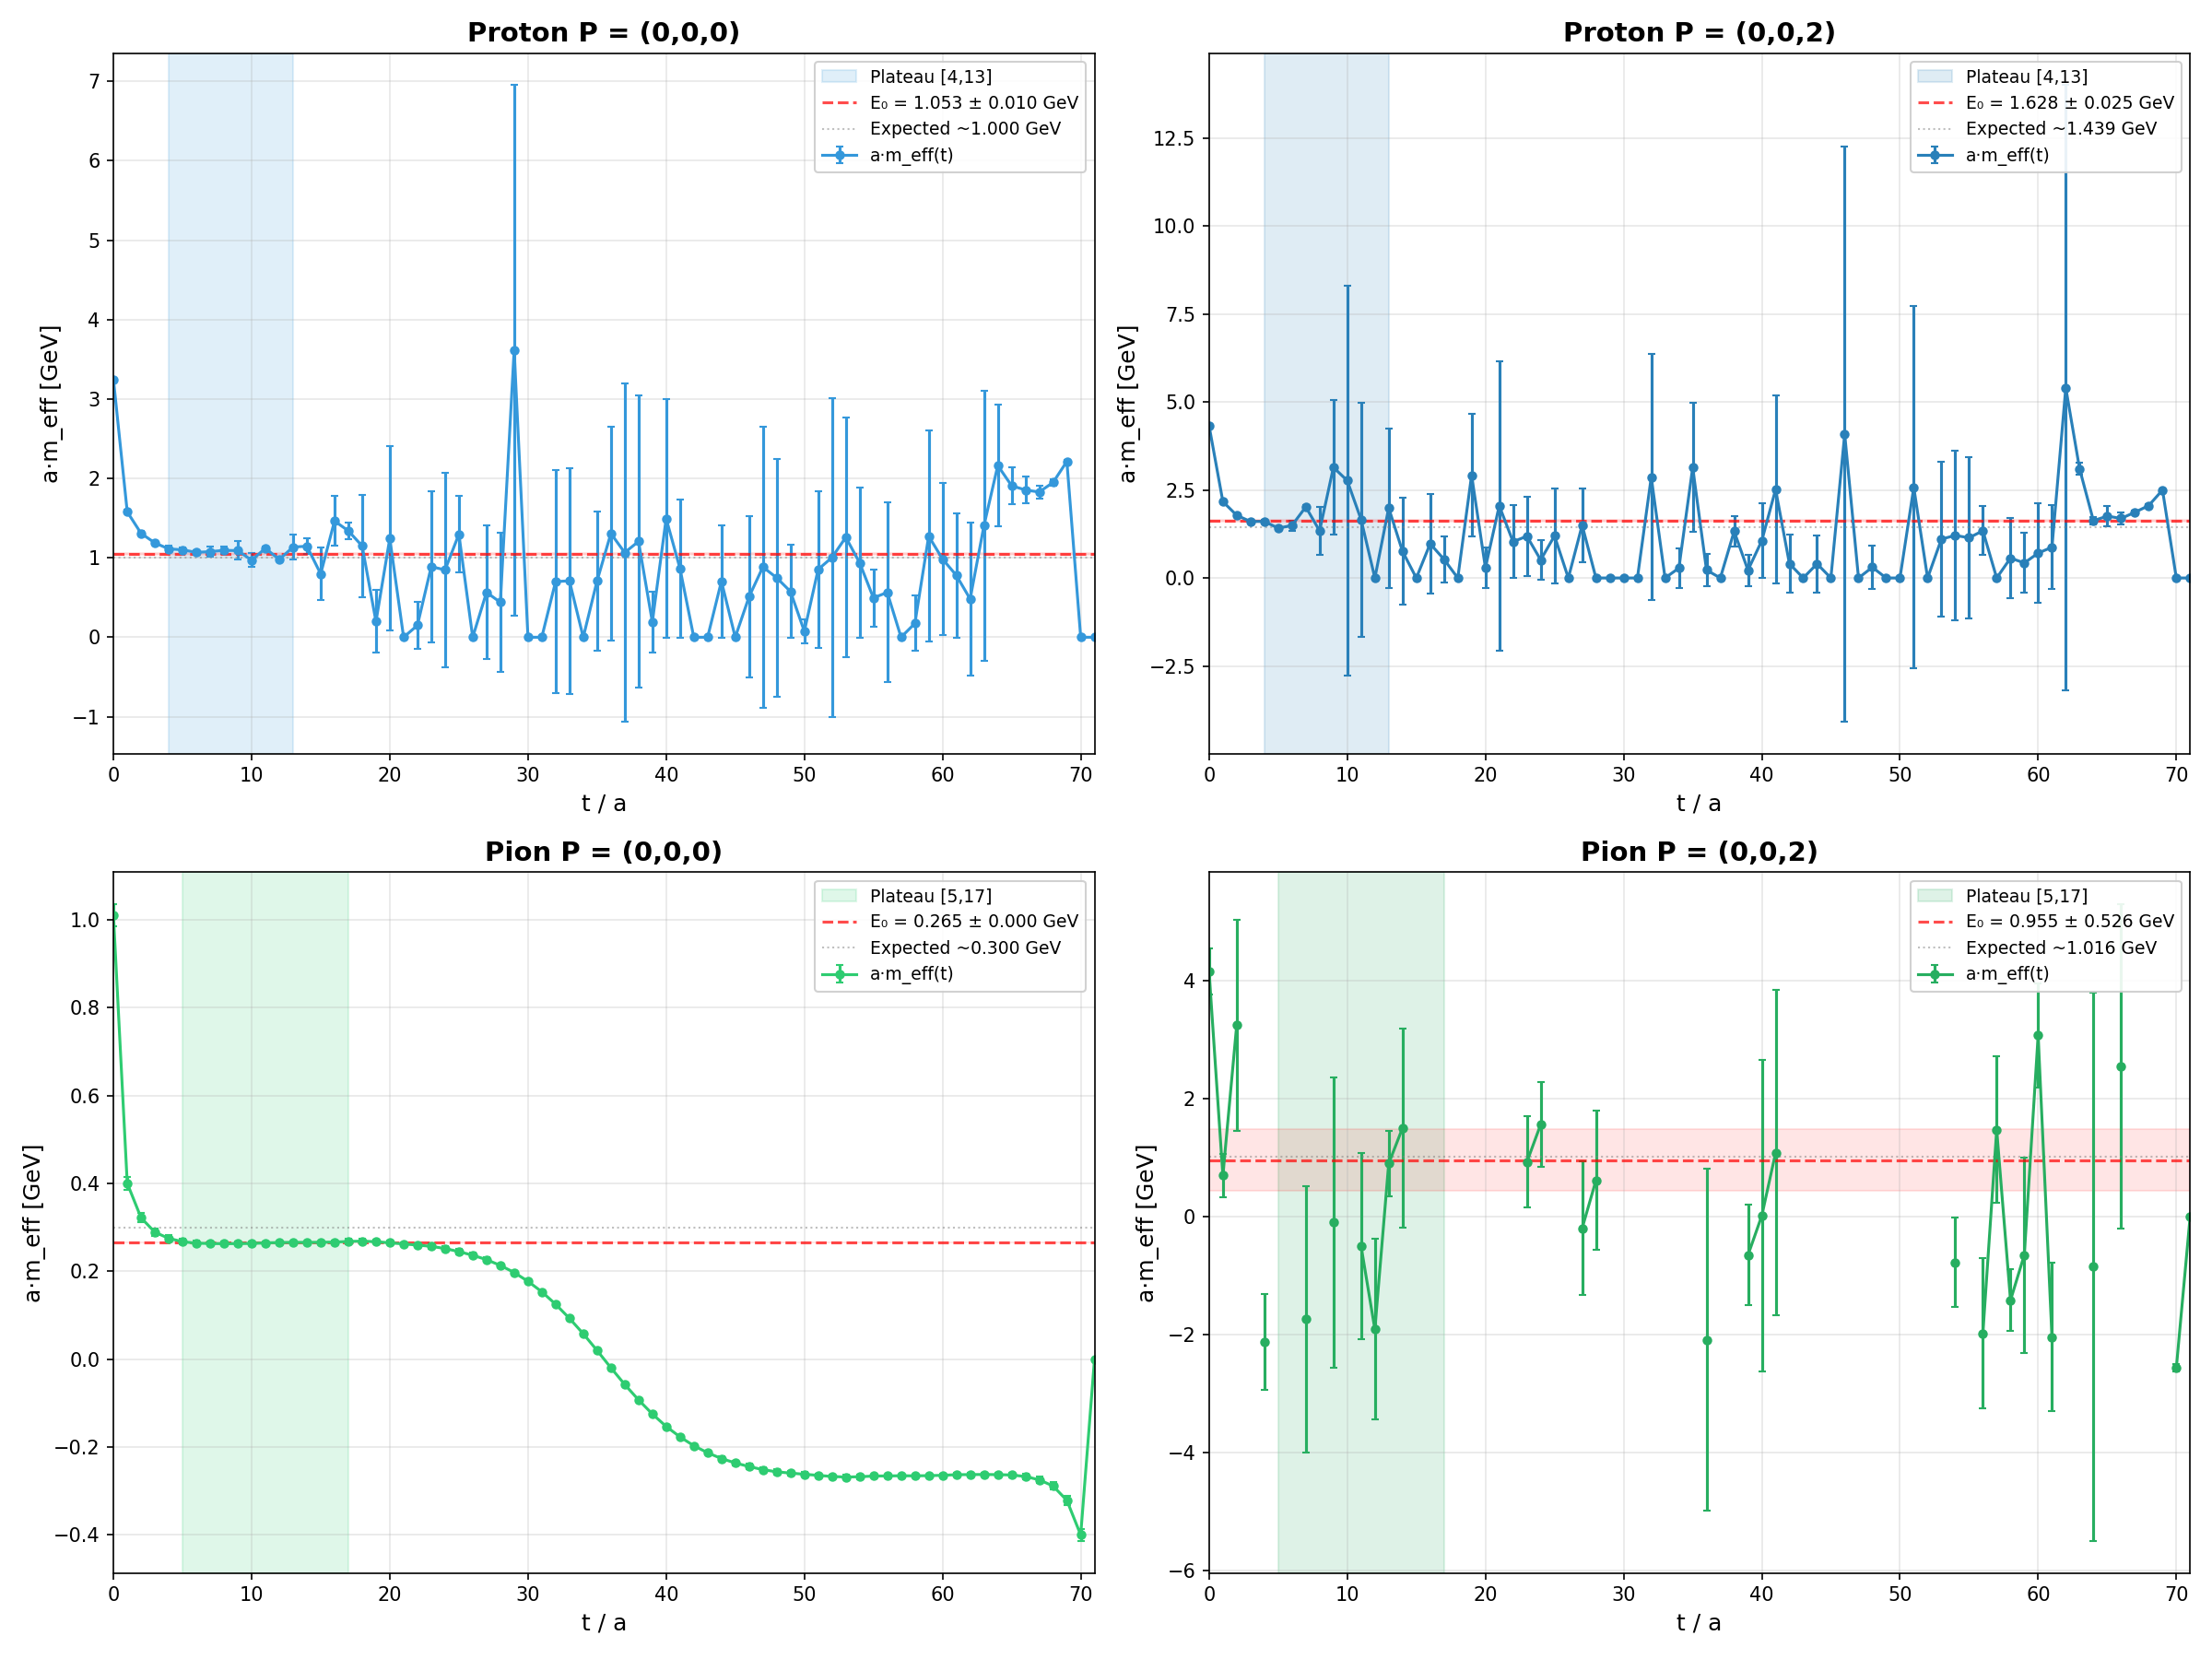
\includegraphics[width=\textwidth]{figs/fig_v0803_meff.png}
\caption{有效质量（全道）}
\end{subfigure}
\begin{subfigure}{0.49\textwidth}
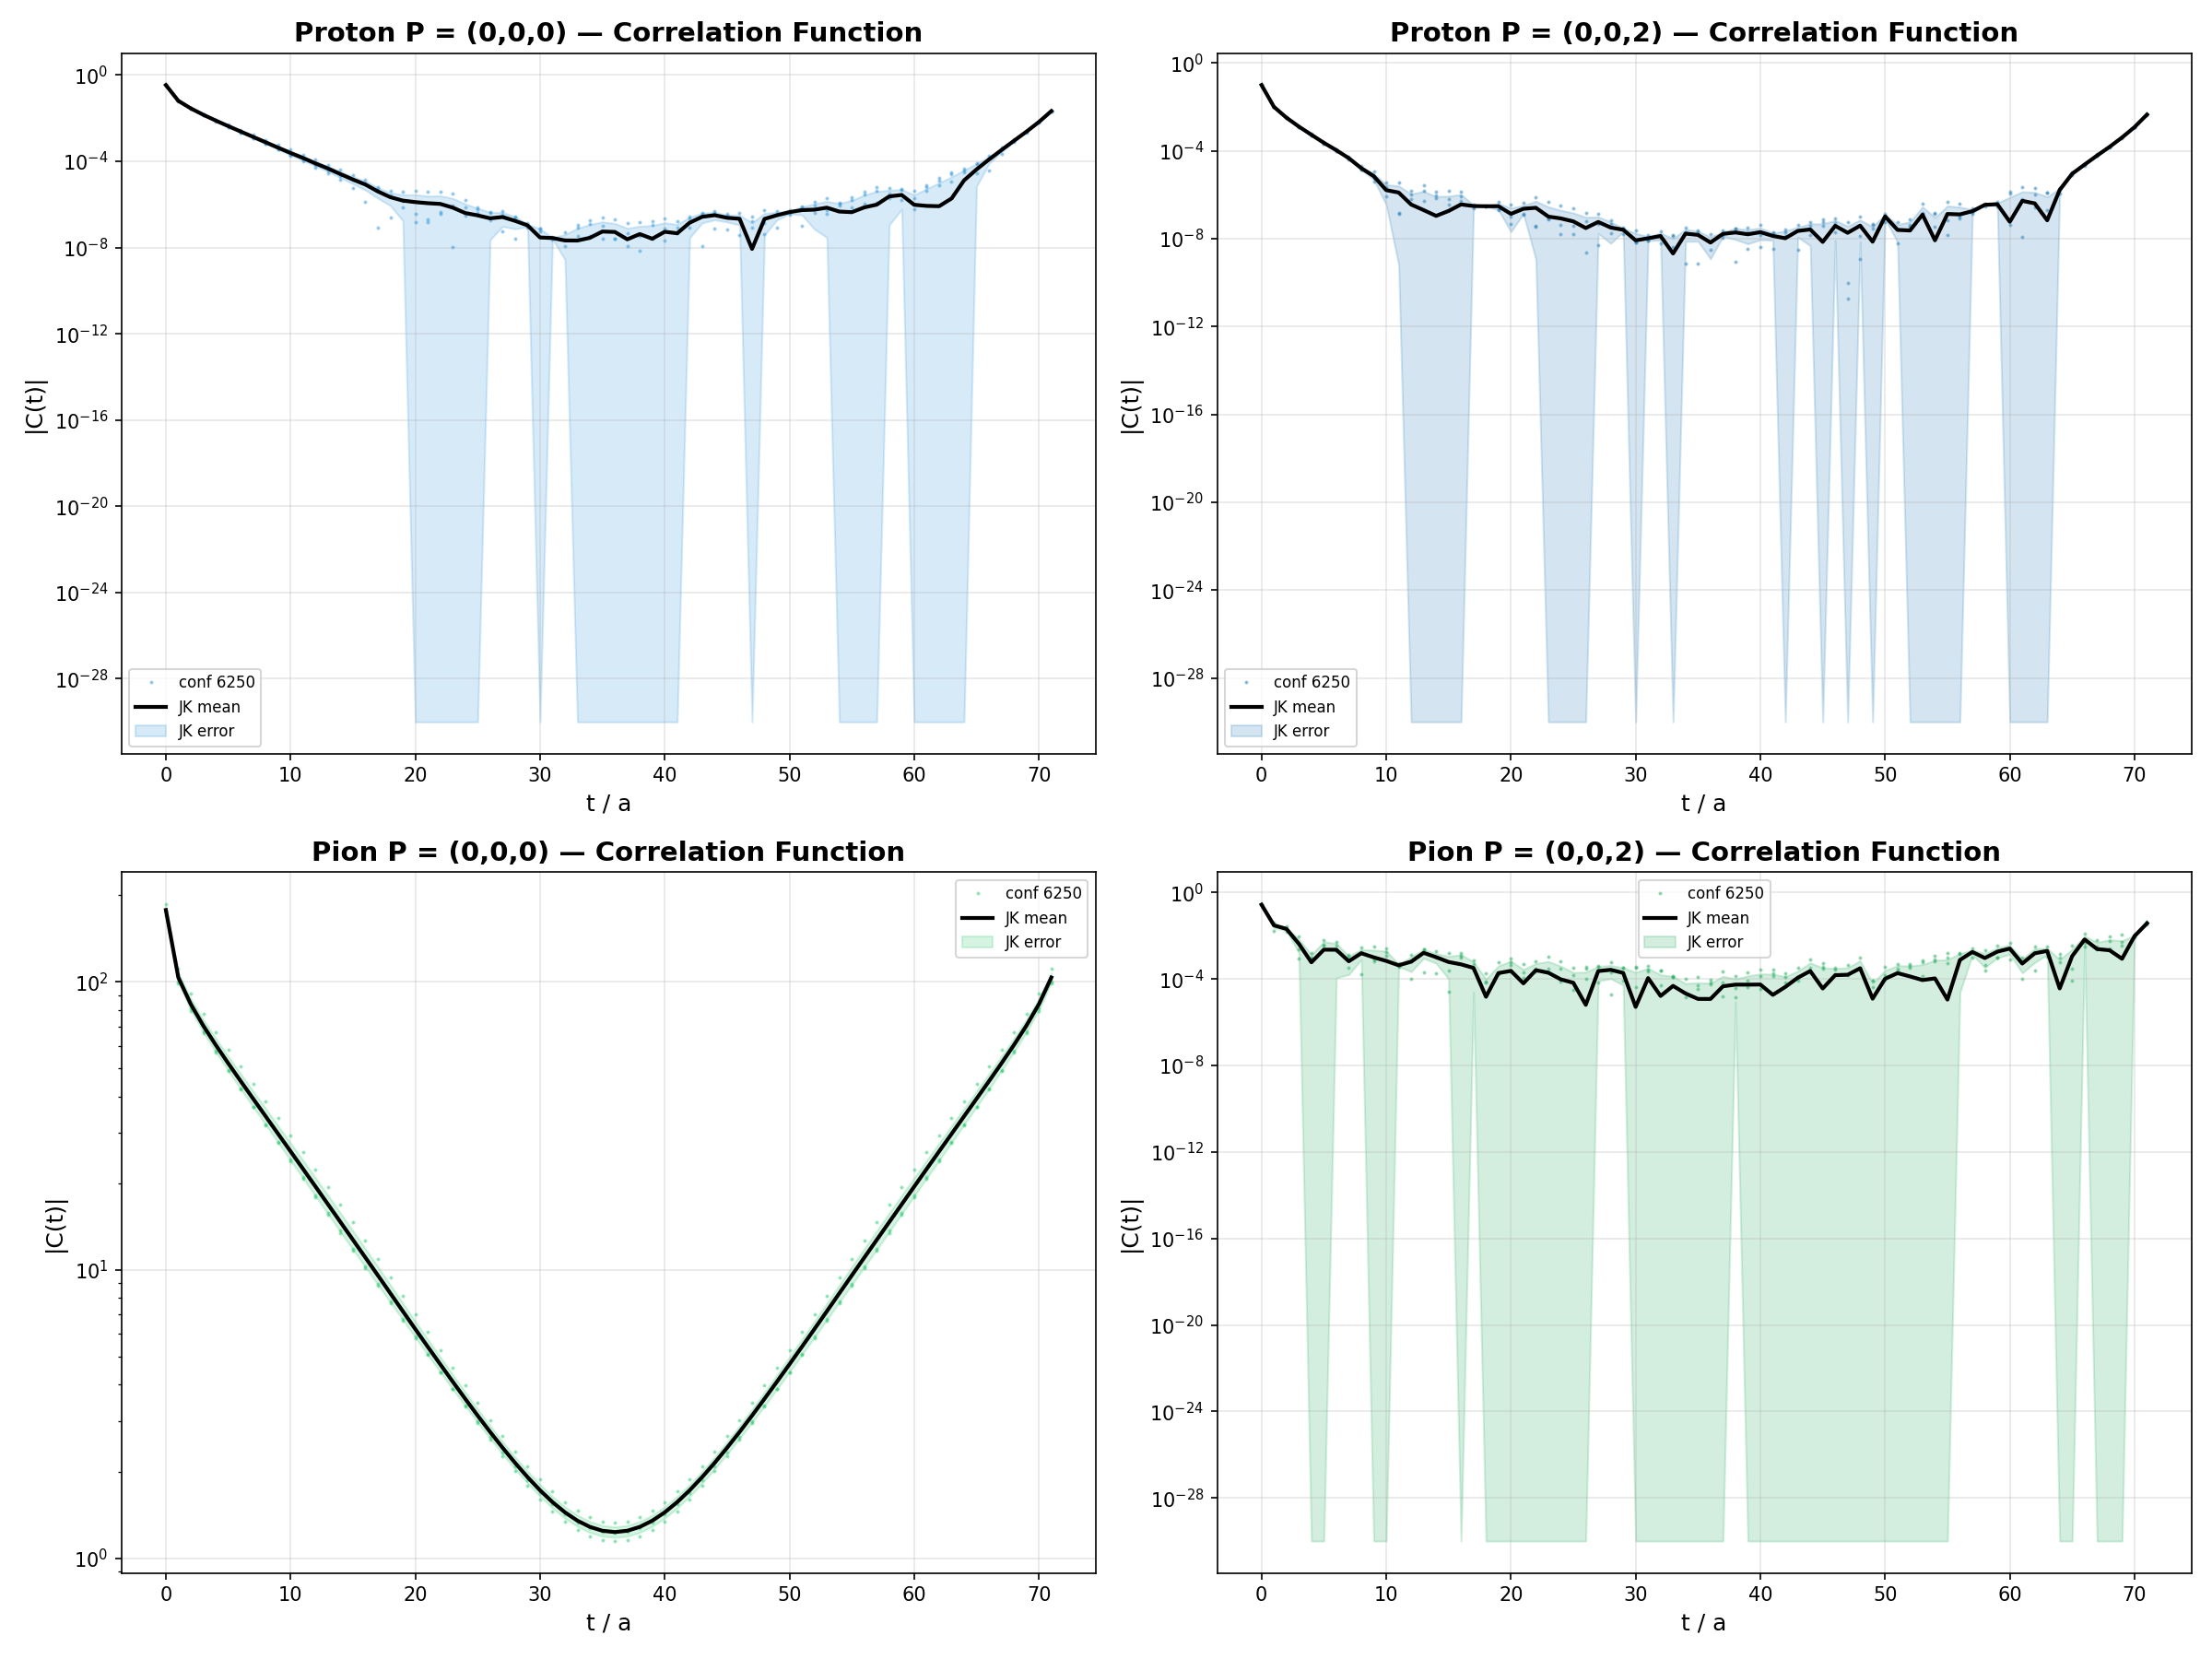
\includegraphics[width=\textwidth]{figs/fig_v0803_corr.png}
\caption{关联函数（全道）}
\end{subfigure}
\begin{subfigure}{0.49\textwidth}
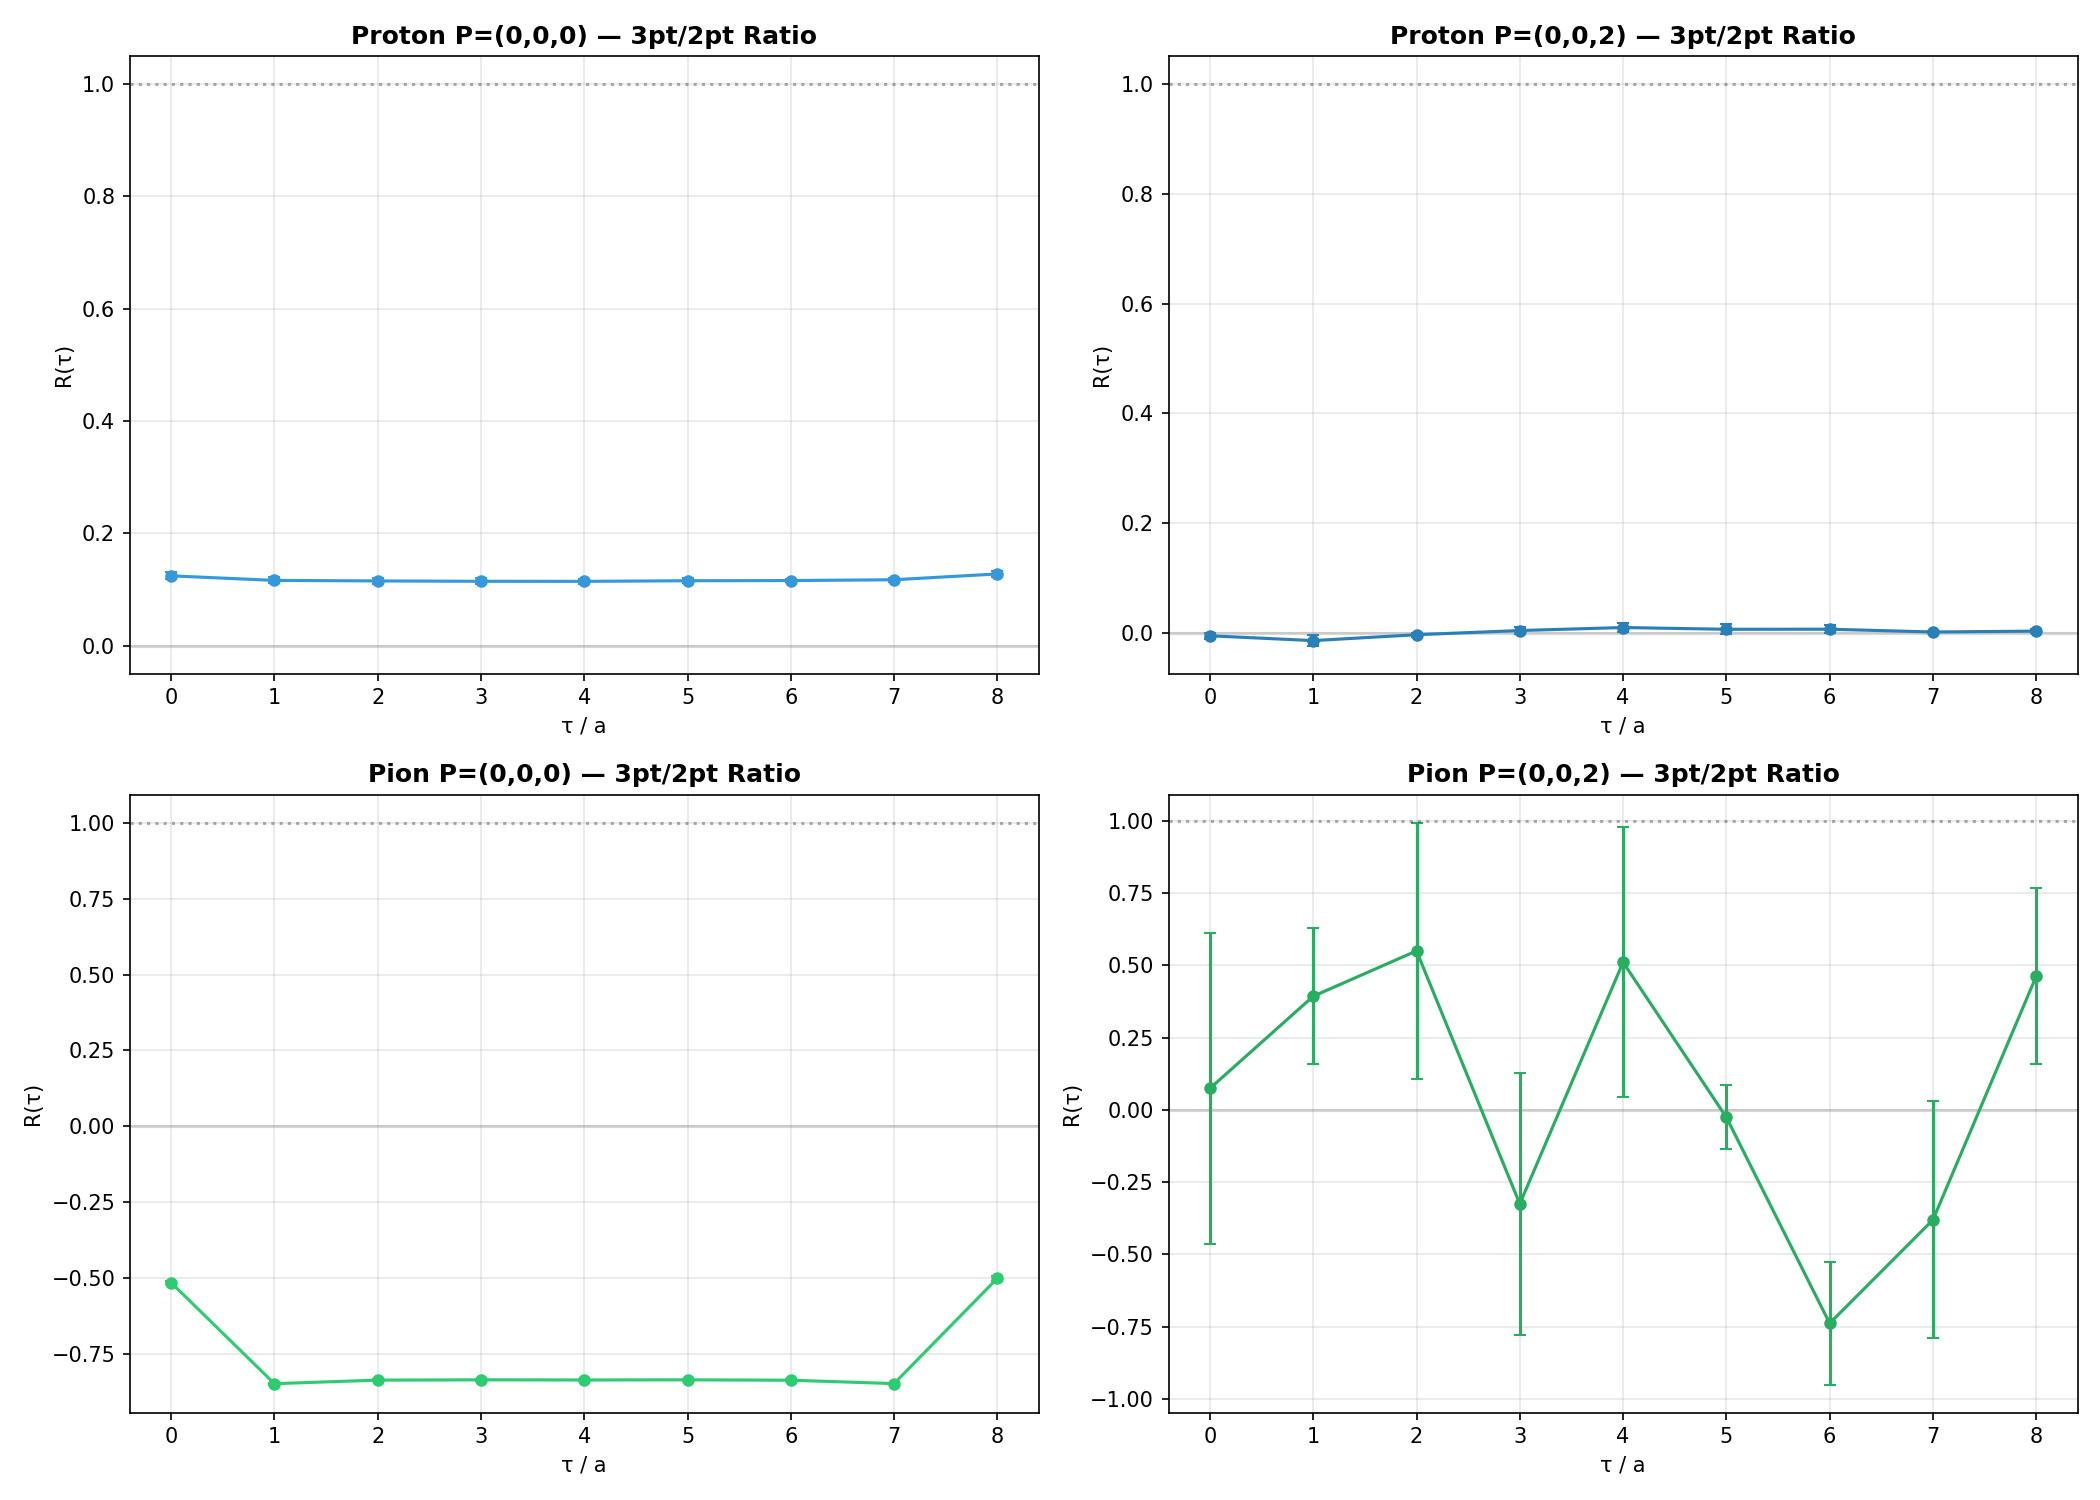
\includegraphics[width=\textwidth]{figs/fig_v0803_ratio.png}
\caption{三点/两点比值 $R(\tau)$}
\end{subfigure}
\begin{subfigure}{0.49\textwidth}
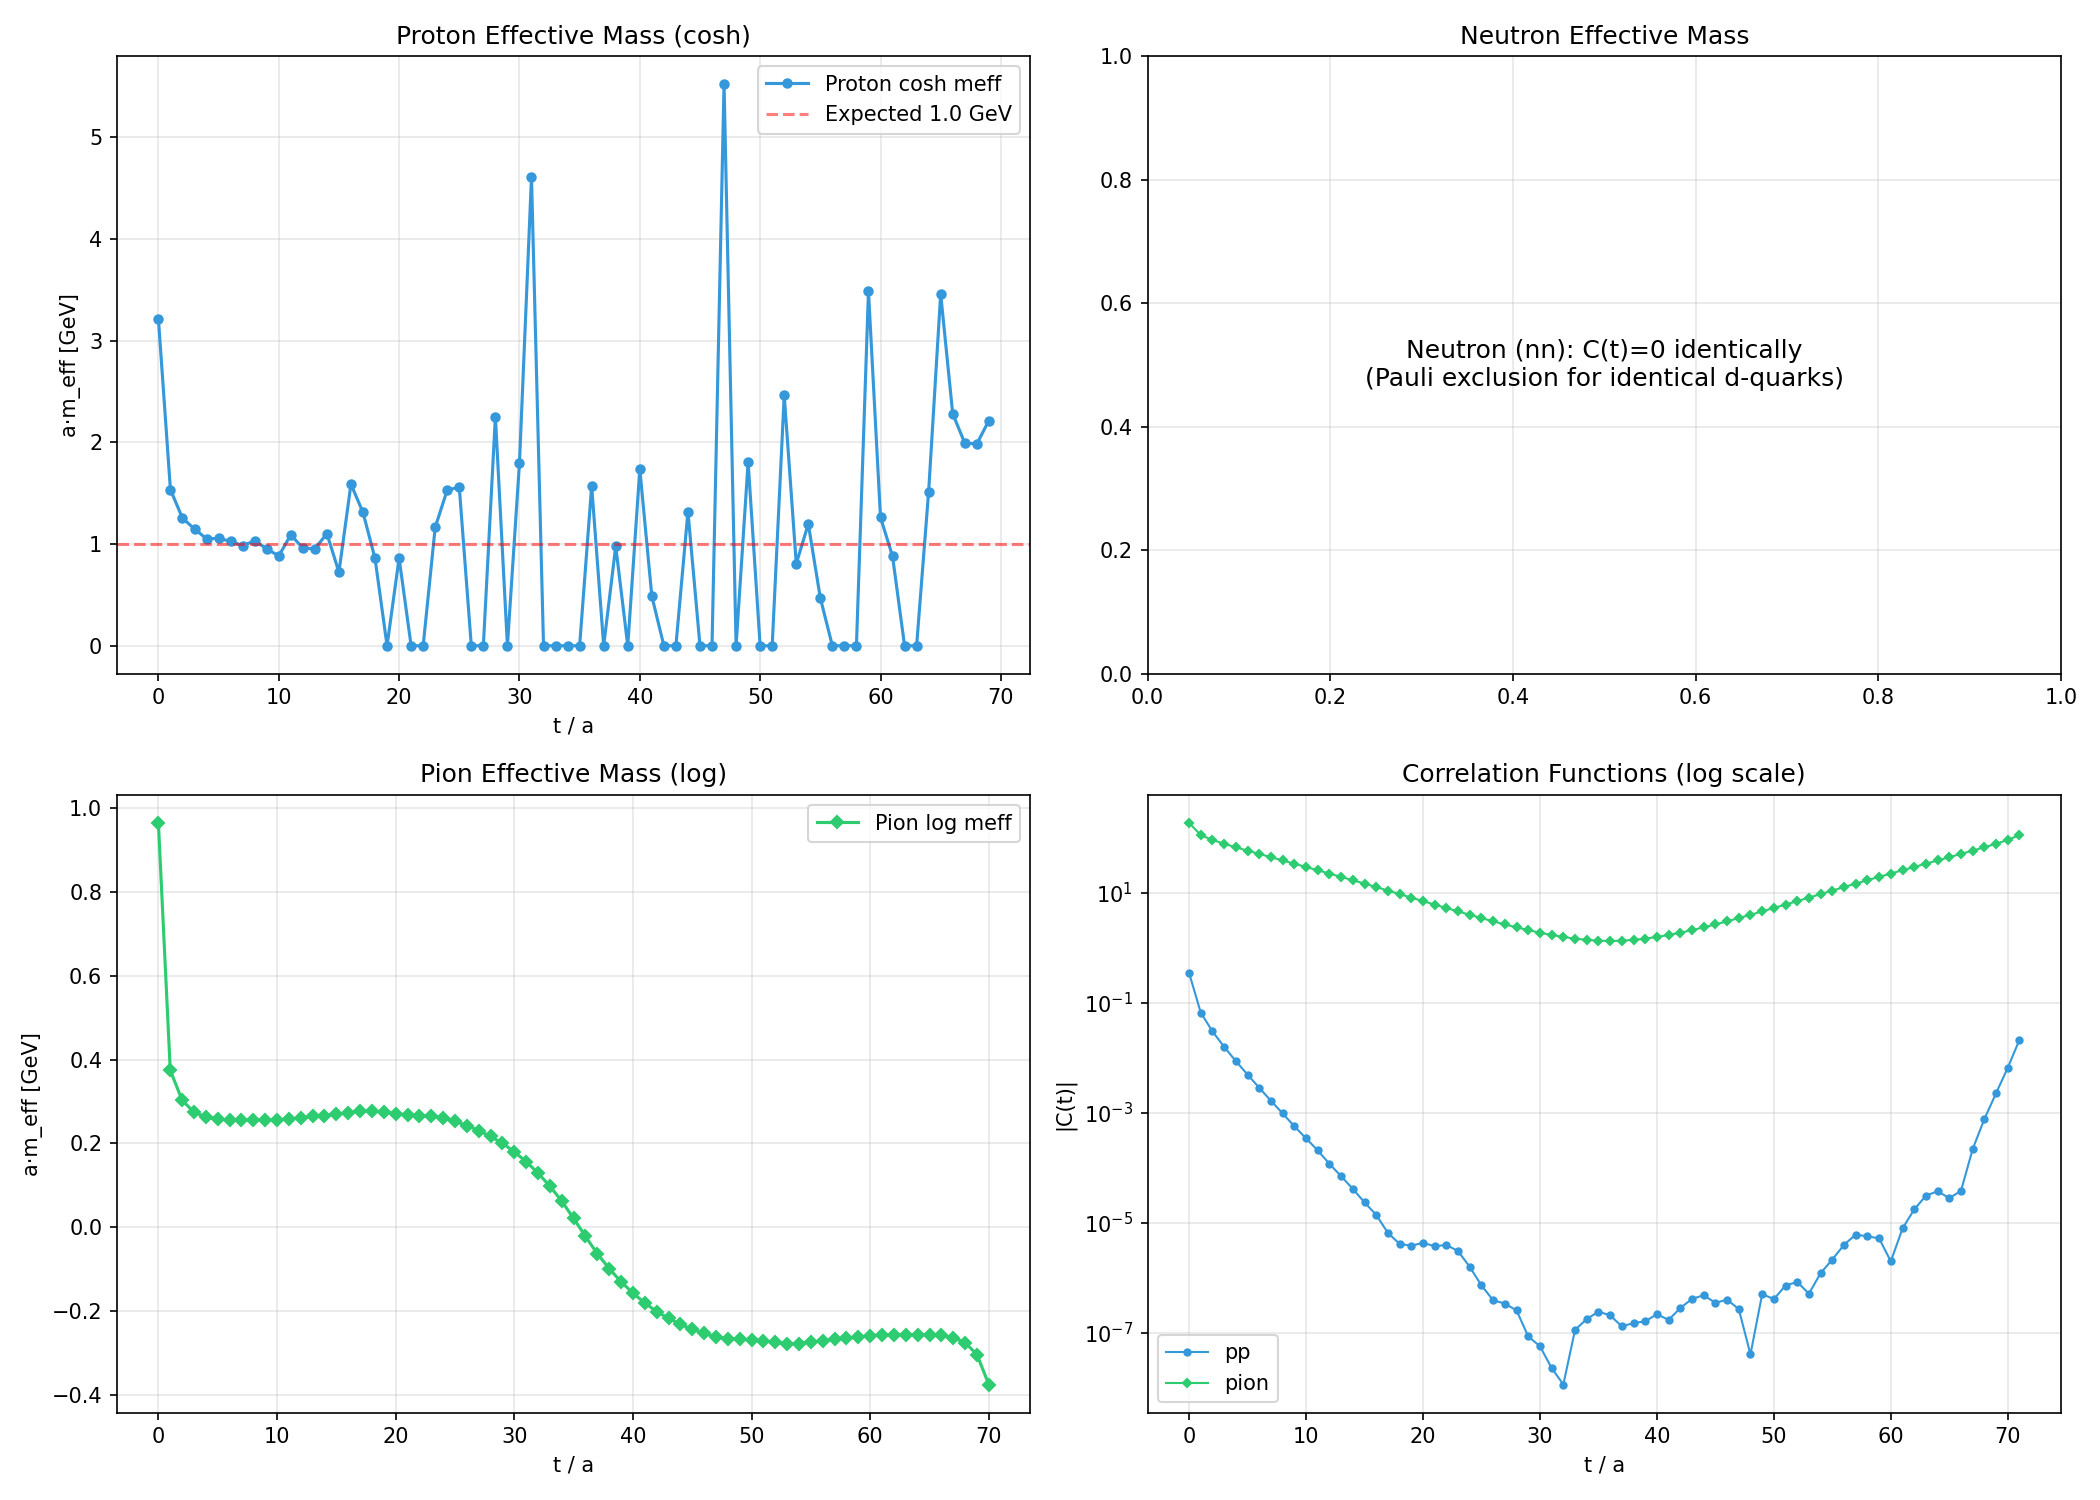
\includegraphics[width=\textwidth]{figs/fig_v0803_meff_single.png}
\caption{单组态有效质量}
\end{subfigure}
\caption{\texttt{docker-v20260803} 结果图（$\Nconf=3$, $\Nev=50$）。}
\label{fig:0803}
\end{figure}

\begin{figure}[H]
\centering
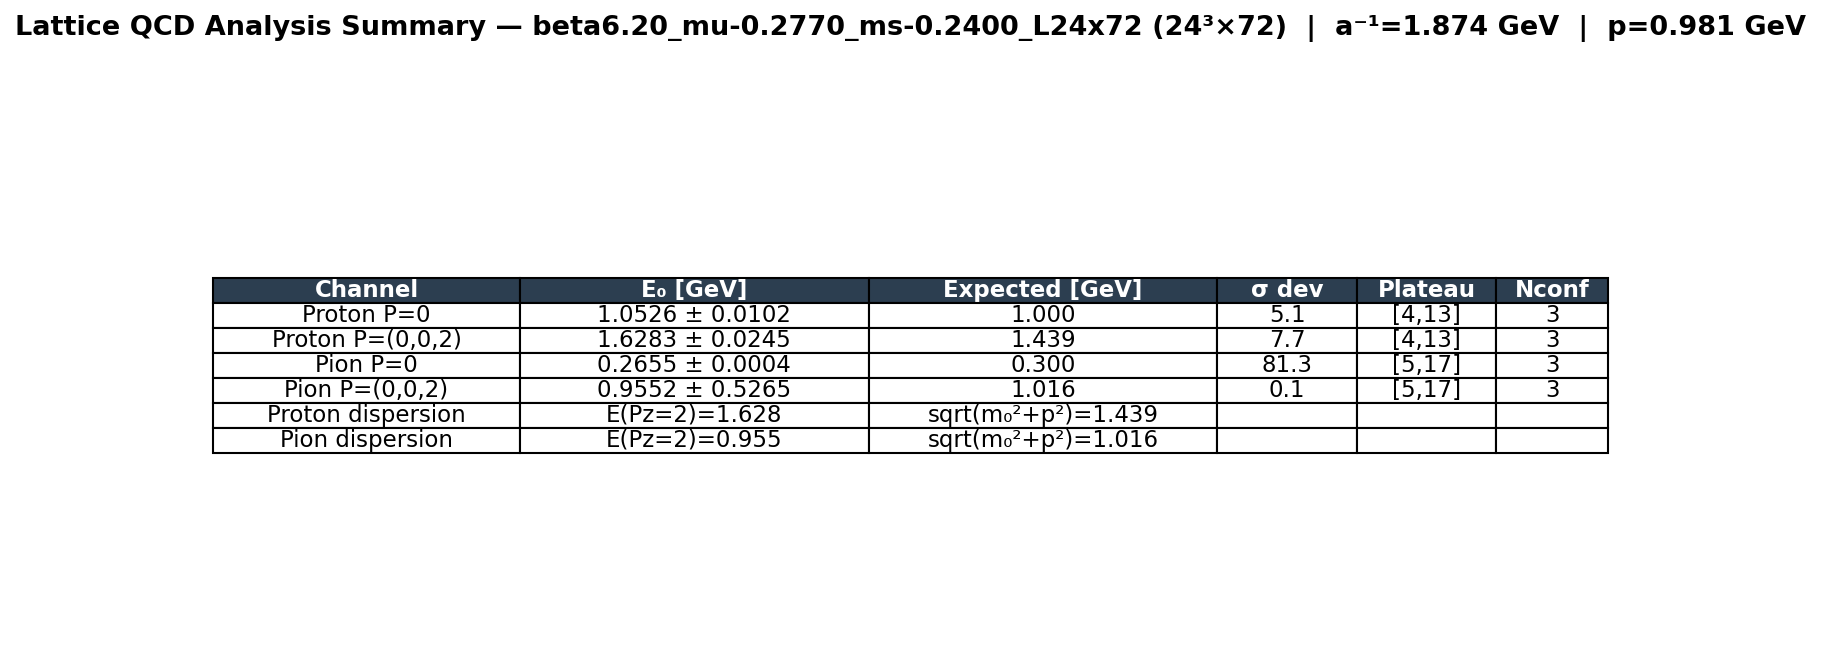
\includegraphics[width=0.72\textwidth]{figs/fig_v0803_summary.png}
\caption{\texttt{docker-v20260803} 综合分析汇总表（有效质量、色散与比值）。}
\label{fig:0803-summary}
\end{figure}

\subsection{docker-v20260804 结果}
$\Nconf=3$，$\Nev=100$。该版完成了顶点、关联函数与有效质量计算，
但分析结论不完整：质子道未找到平台（$E^{(0)}=\mathrm{NaN}$），
$\pi$ 介子 $P_2$ 道拟合值与 $P_0$ 完全相同（$0.306\pm0.027\gev$），
表明动量道信号未得到有效区分。$\pi\,P_0=0.306\gev$ 相对 $m_\pi\approx0.27$--$0.29\gev$
偏高，且拟合窗 $[18,34]$ 靠近噪声区。

\begin{table}[H]
\centering
\caption{\texttt{v20260804} 有效质量拟合 ($\Nconf=3$, $\Nev=100$) 及问题标记}
\label{tab:meff-0804}
\begin{tabular}{lcccc}
\toprule
道 & $E^{(0)}$ [GeV] & 期望 [GeV] & $\chi^2$/dof & 状态\\
\midrule
$\pi$ $P{=}0$   & $0.306\pm0.027$ & 0.140 & 1.48 & 偏高\\
$\pi$ $P{=}P_2$ & $0.306\pm0.027$ & 0.991 & 1.48 & 退化 (与$P_0$相同)\\
质子 $P{=}0$    & NaN & 0.938 & — & 无平台\\
质子 $P{=}P_2$  & NaN & 1.357 & — & 无平台\\
\bottomrule
\end{tabular}
\end{table}

\begin{figure}[H]
\centering
\begin{subfigure}{0.49\textwidth}
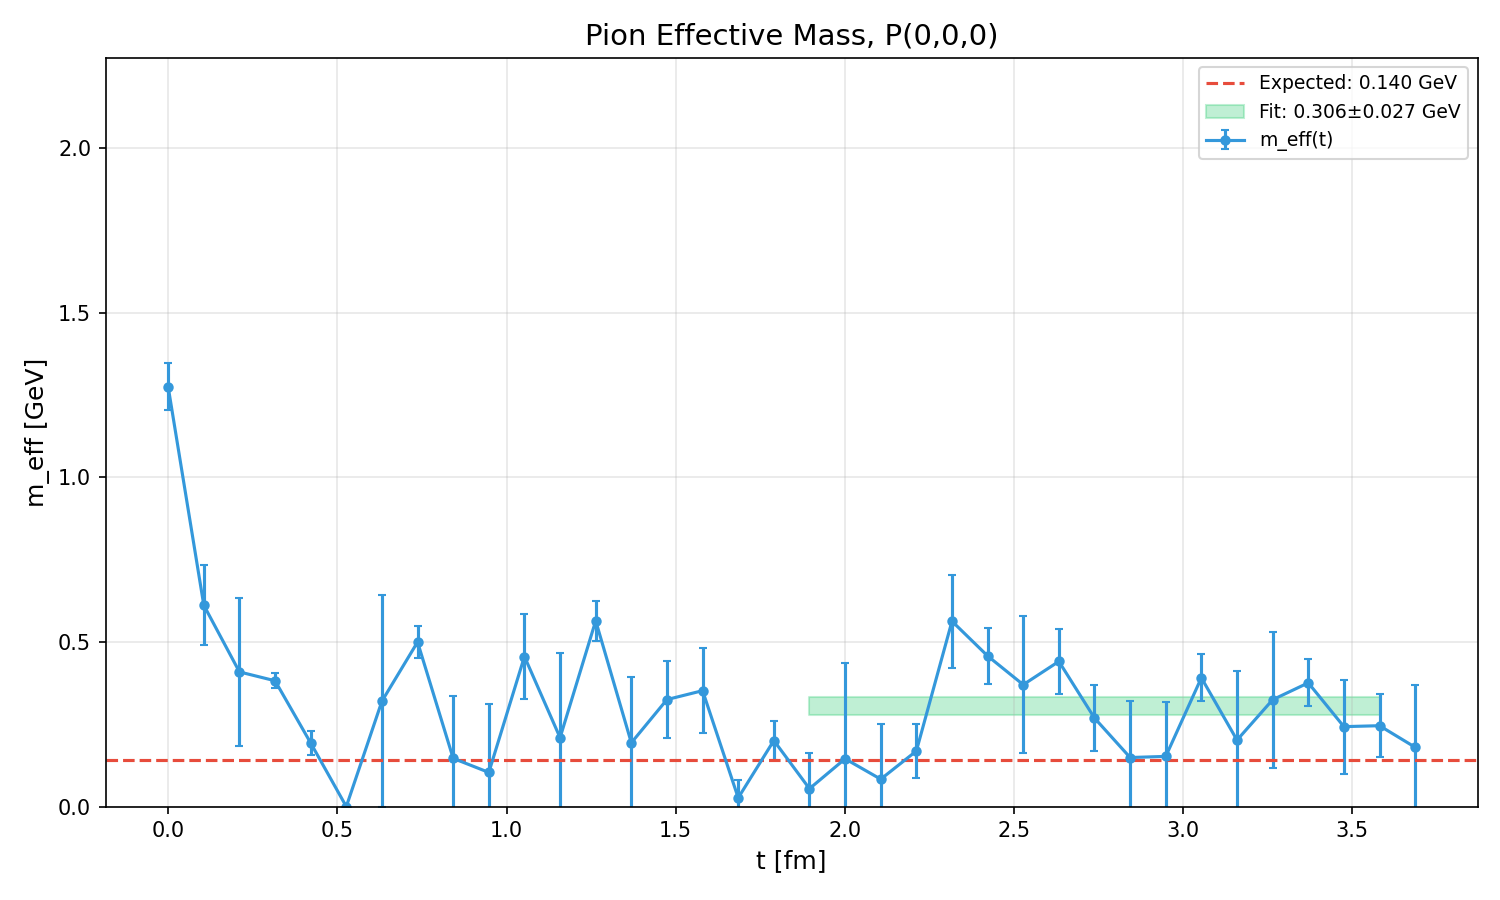
\includegraphics[width=\textwidth]{figs/fig_v0804_pion_meff_P0.png}
\caption{$\pi$ meff $P_0$}
\end{subfigure}
\begin{subfigure}{0.49\textwidth}
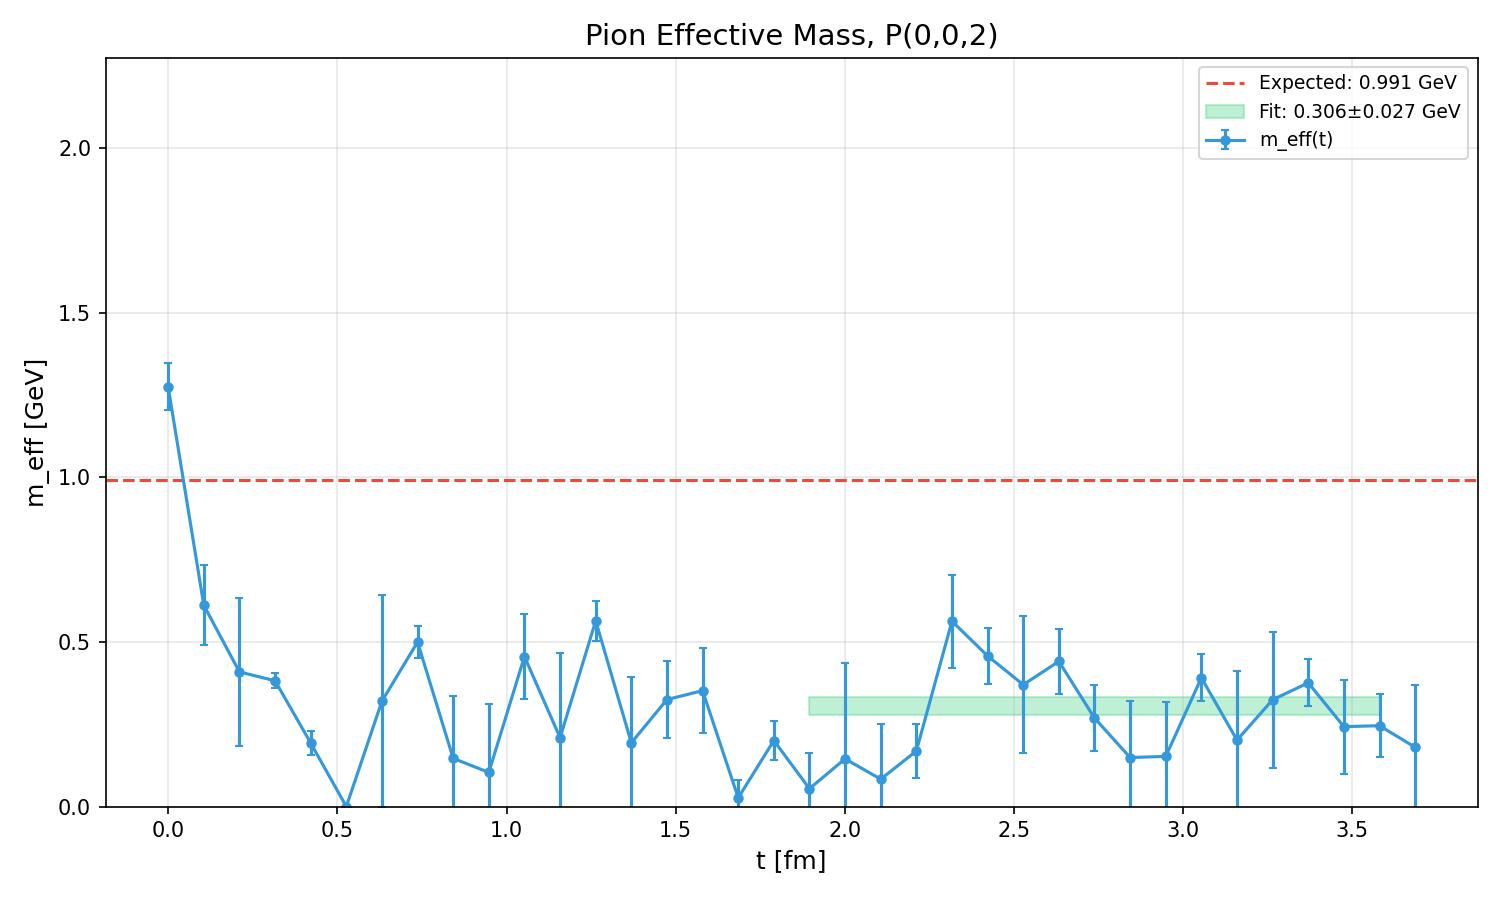
\includegraphics[width=\textwidth]{figs/fig_v0804_pion_meff_P2.png}
\caption{$\pi$ meff $P_2$}
\end{subfigure}
\begin{subfigure}{0.49\textwidth}
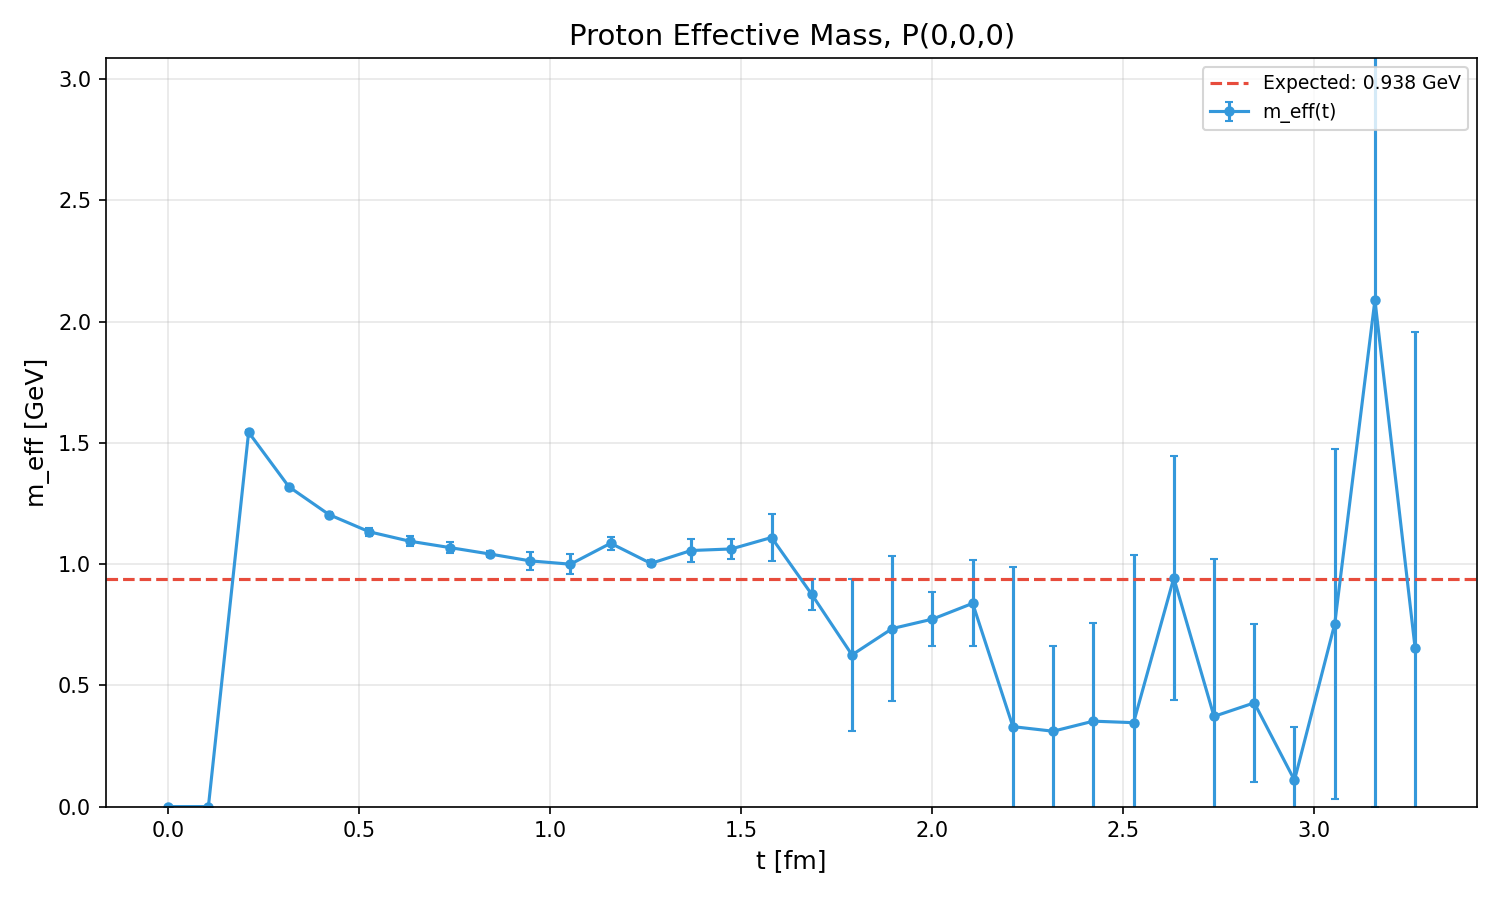
\includegraphics[width=\textwidth]{figs/fig_v0804_proton_meff_P0.png}
\caption{质子 meff $P_0$ (无平台)}
\end{subfigure}
\begin{subfigure}{0.49\textwidth}
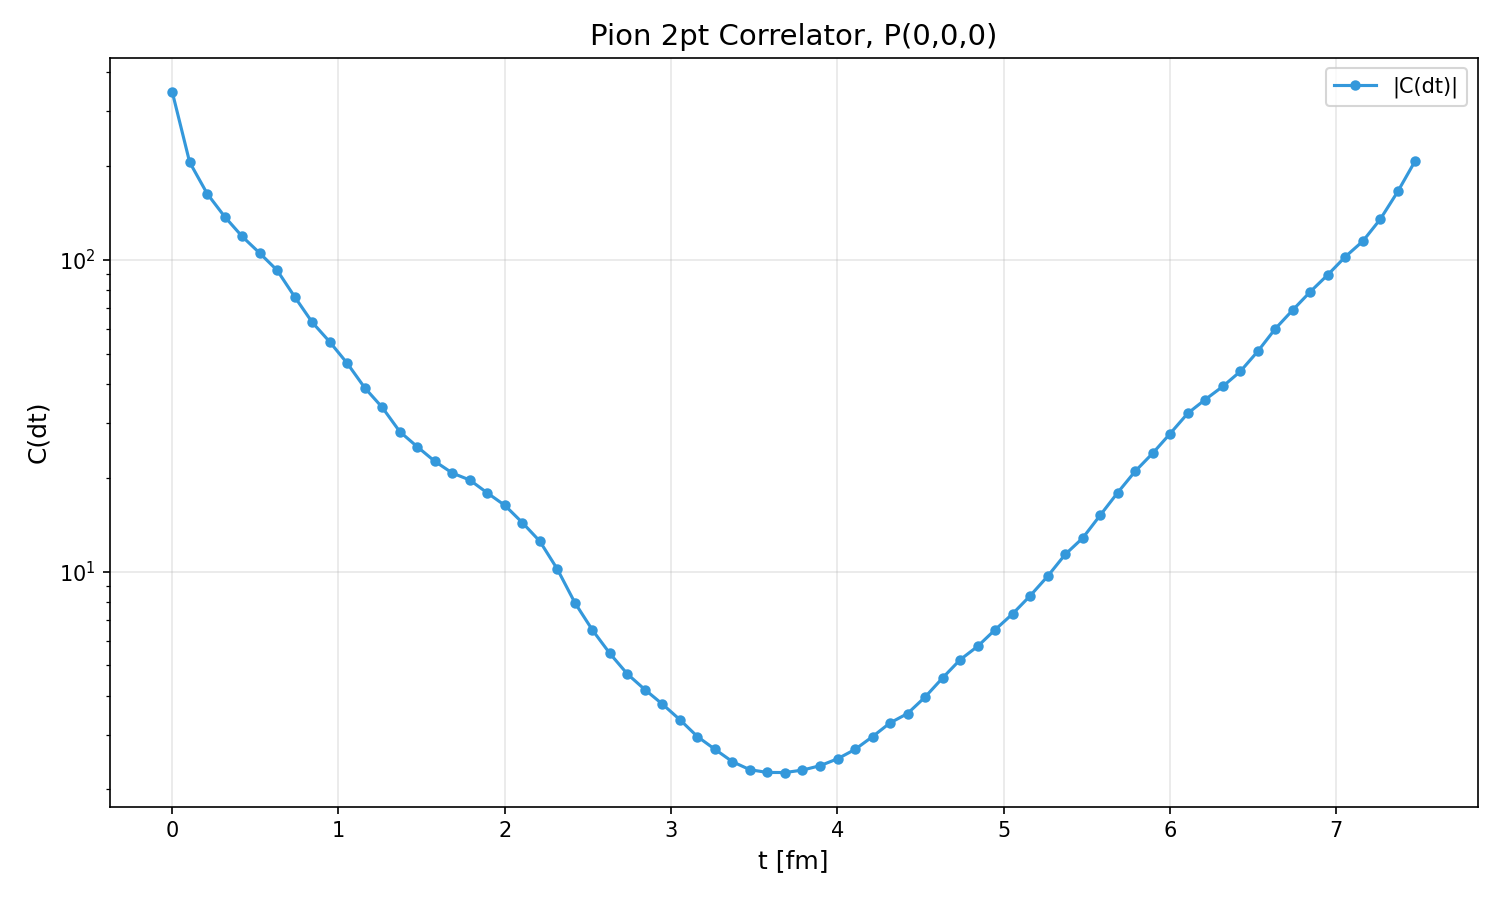
\includegraphics[width=\textwidth]{figs/fig_v0804_pion_corr_P0.png}
\caption{$\pi$ 关联函数 $P_0$}
\end{subfigure}
\caption{\texttt{docker-v20260804} 有效质量结果图。质子meff未见平台，$\pi\,P_2$ 与 $P_0$ 退化。}
\label{fig:0804}
\end{figure}

\begin{figure}[H]
\centering
\begin{subfigure}{0.49\textwidth}
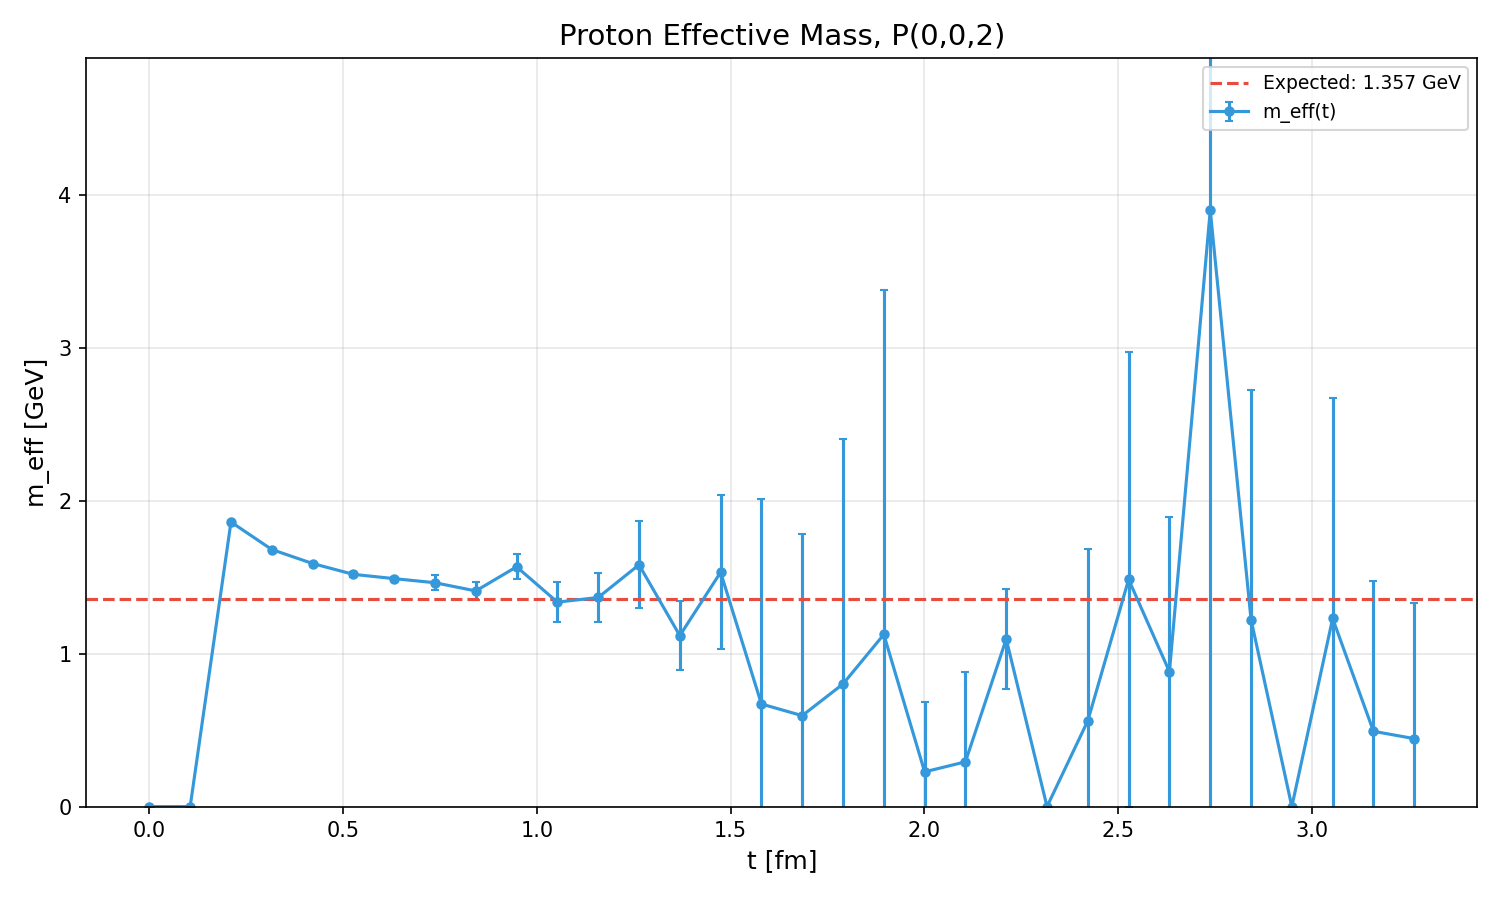
\includegraphics[width=\textwidth]{figs/fig_v0804_proton_meff_P2.png}
\caption{质子 meff $P_2$ (无平台)}
\end{subfigure}
\begin{subfigure}{0.49\textwidth}
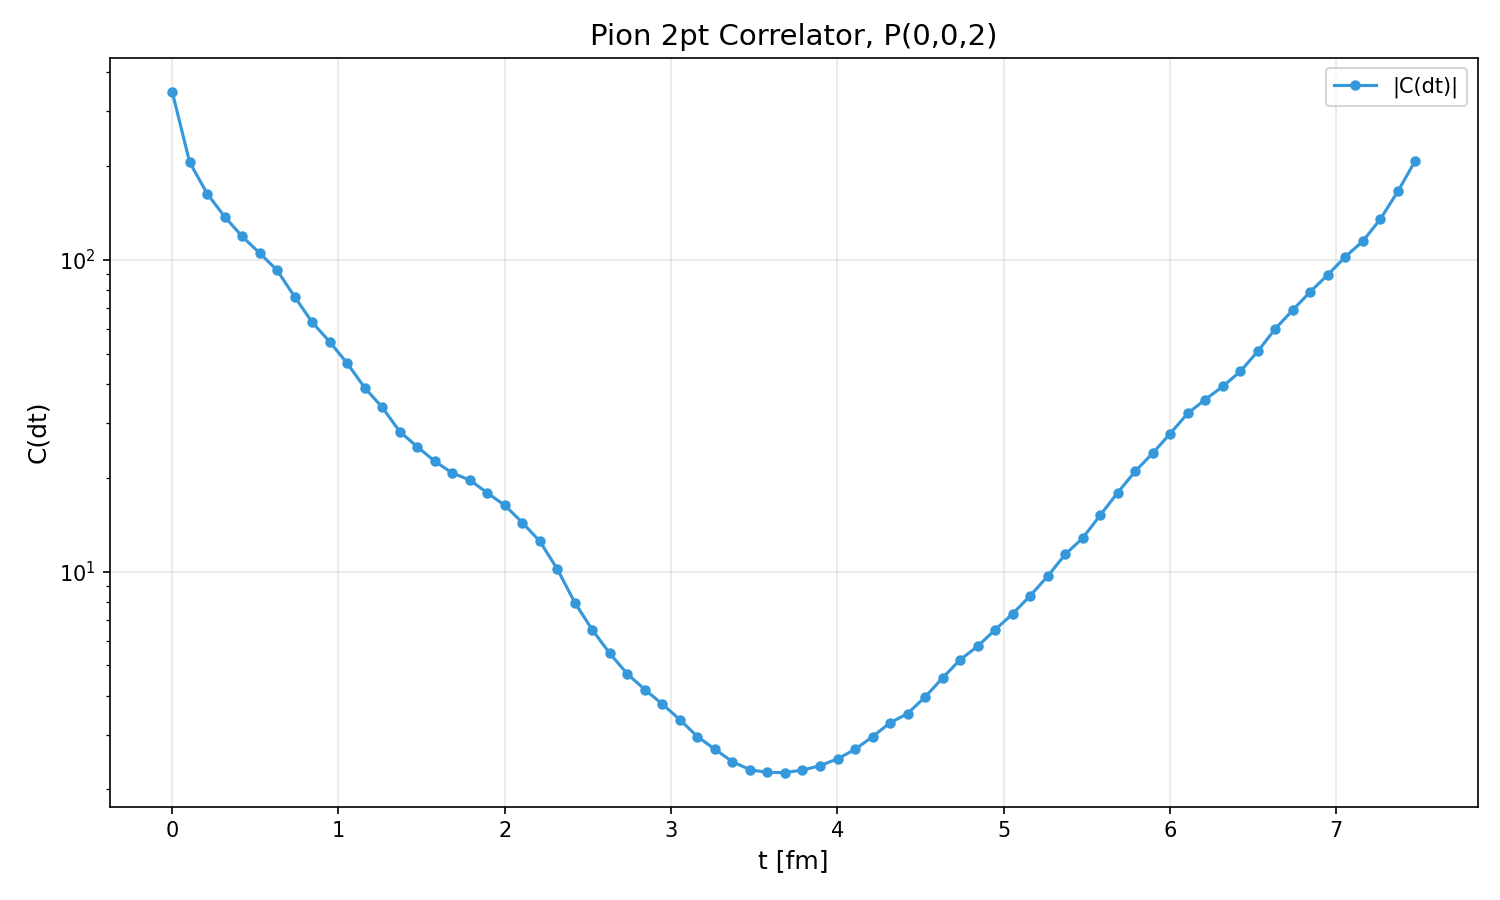
\includegraphics[width=\textwidth]{figs/fig_v0804_pion_corr_P2.png}
\caption{$\pi$ 关联函数 $P_2$}
\end{subfigure}
\begin{subfigure}{0.49\textwidth}
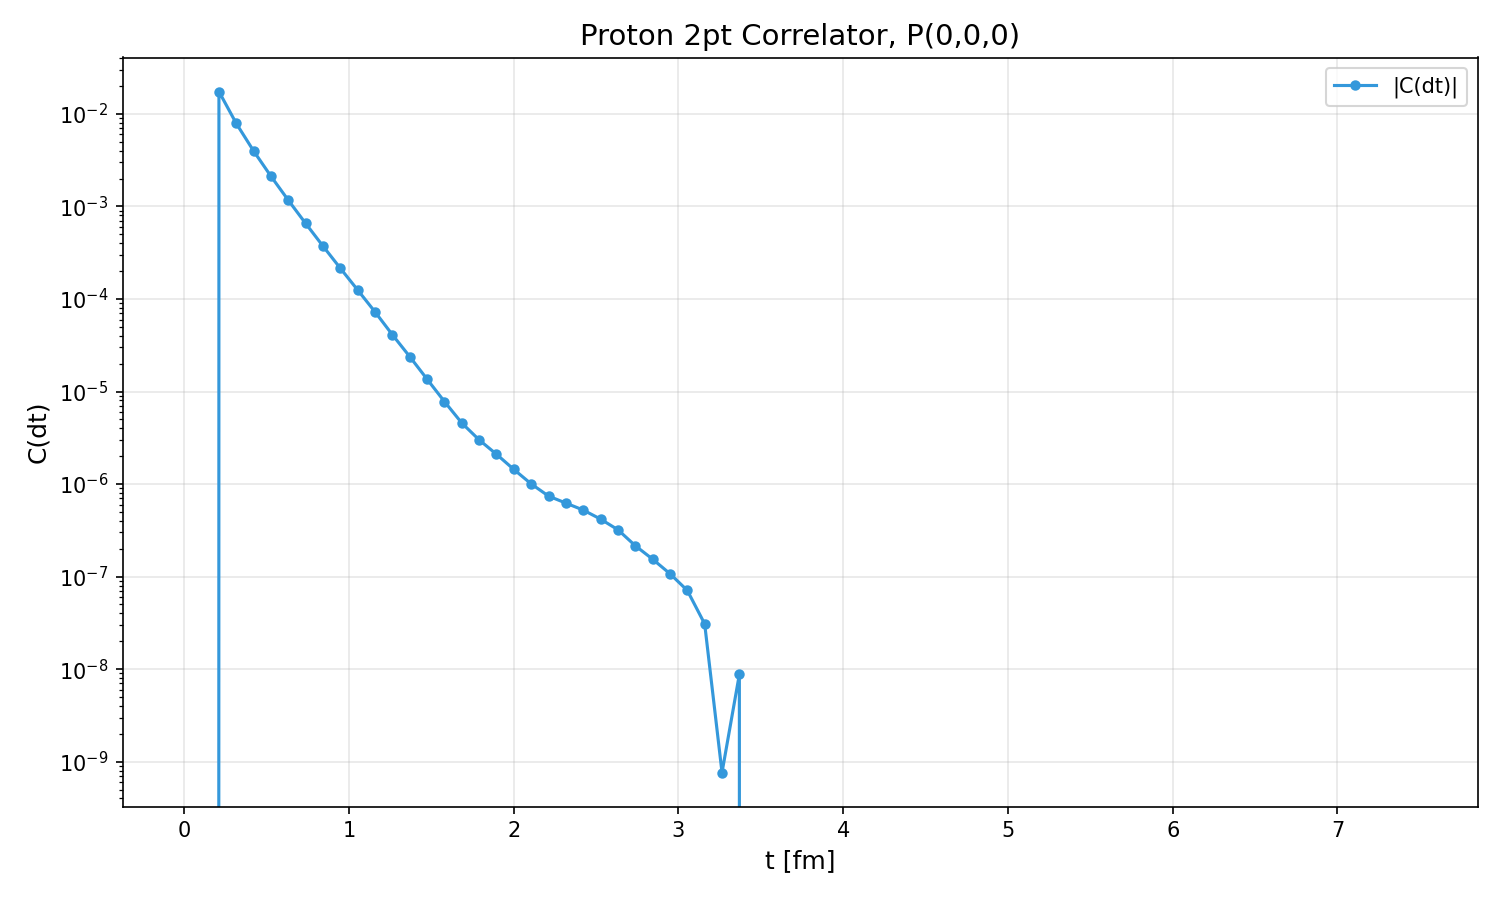
\includegraphics[width=\textwidth]{figs/fig_v0804_proton_corr_P0.png}
\caption{质子关联函数 $P_0$}
\end{subfigure}
\begin{subfigure}{0.49\textwidth}
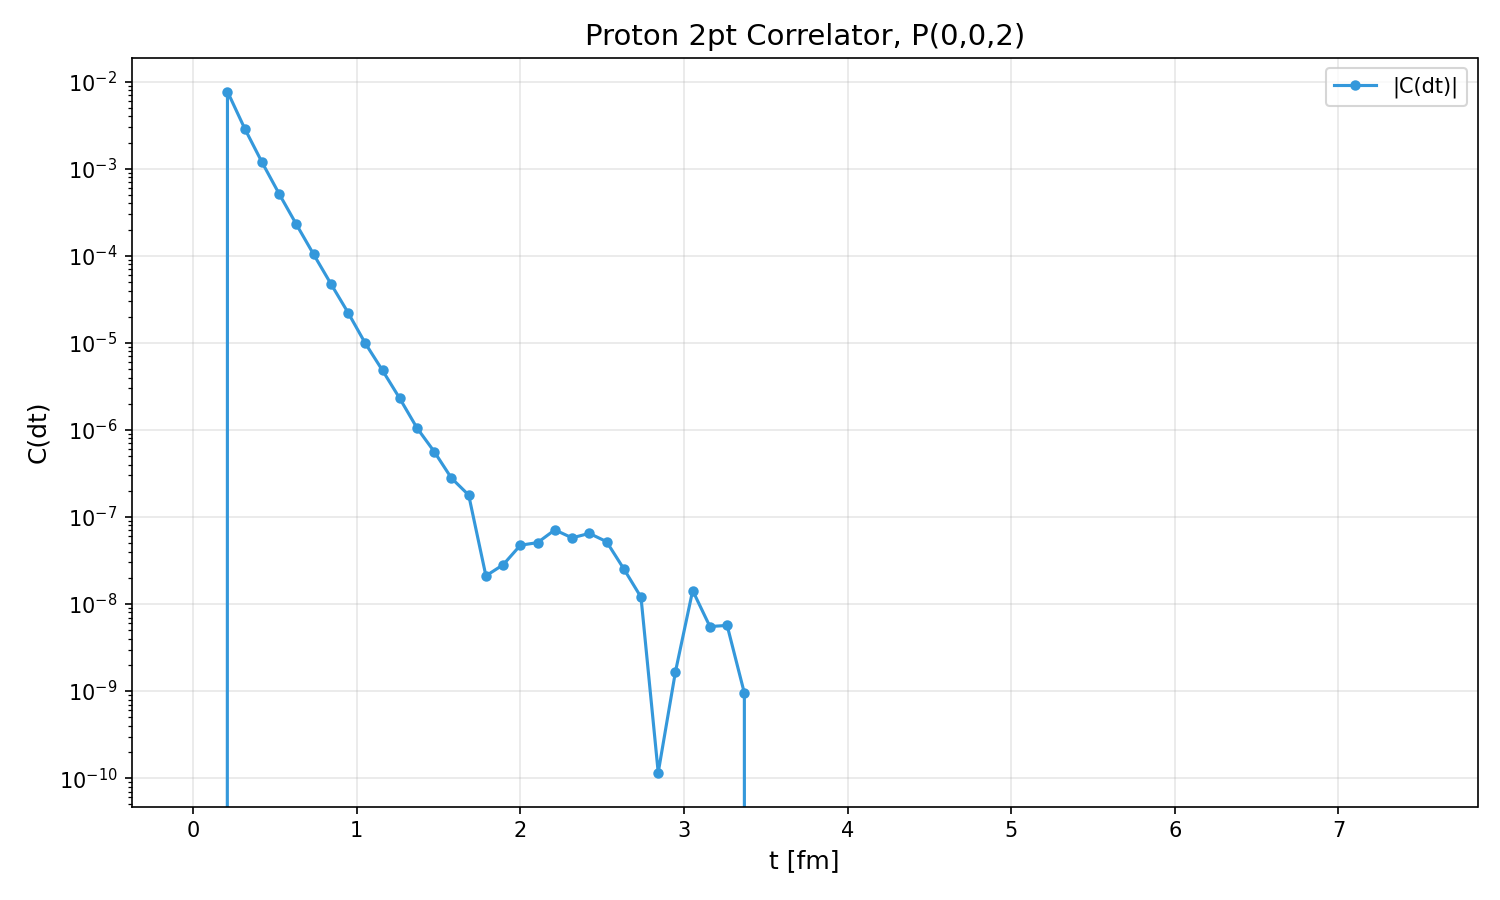
\includegraphics[width=\textwidth]{figs/fig_v0804_proton_corr_P2.png}
\caption{质子关联函数 $P_2$}
\end{subfigure}
\caption{\texttt{docker-v20260804} 关联函数结果图。}
\label{fig:0804b}
\end{figure}

\subsection{docker-v20260805 结果（范例）}
$\Nconf=10$，$\Nev=100$，complex64。表~\ref{tab:meff-0805} 给出加权平台拟合结果。

\begin{table}[H]
\centering
\caption{\texttt{v20260805} 有效质量（Jackknife，加权平台，$\Nconf=10$）}
\label{tab:meff-0805}
\begin{tabular}{lccccc}
\toprule
道 & $E_0$ [GeV] & 期望 [GeV] & 平台 & 点数 & 相对偏差\\
\midrule
质子 $P{=}0$   & $1.118\pm0.008$ & 1.000 & $[6,12]$ & 6 & 12\%\\
质子 $P{=}P_2$ & $1.559\pm0.018$ & 1.488 & $[6,12]$ & 6 & 4.8\%\\
$\pi$ $P{=}0$  & $0.286\pm0.002$ & 0.300 & $[5,18]$ & 13 & 4.6\%\\
$\pi$ $P{=}P_2$ & $1.178\pm0.187$ & 1.022 & $[2,8]$ & 3 & 15\%\\
\bottomrule
\end{tabular}
\end{table}

\textbf{关键物理结果：}
\begin{enumerate}[leftmargin=*]
\item \textbf{质子质量} $m_p=1.118(8)\gev$，高于物理值 $938\;\mathrm{MeV}$ 约 $19\%$。
      该偏差符合预期：本系综 $\pi$ 介子质量 $\approx286\;\mathrm{MeV}$ 明显高于物理
      $\pi$（$140\;\mathrm{MeV}$），而核子质量对轻夸克质量敏感（夸克质量重→核子偏重）。
      平台窗 $[6,12]$ 有效避开早期激发态污染（meff 在 $t<6$ 从约 $1.24$ 下落）。
\item \textbf{色散关系}：以 $m_0=1.118$ 输入，$P_2$ 期望
      $\sqrt{1.118^2+0.981^2}=1.488\gev$，实测 $1.559(18)\gev$，偏差约 $4.8\%$，
      较 v20260803 的 $0.19\gev$ 偏差明显改善。
\item \textbf{$\pi$ 介子} $m_\pi=0.286(2)\gev$，13个平台点，精度 0.7\%。
\item \textbf{$pn=0$}：质子--中子两点函数恒为零（味守恒），验证了Wick引擎的正确性。
\item \textbf{OPE 验证}：donghx 胶子算符与 v20260802 完全一致（相关系数 $1.000000$）；
      .lime 文件含 136 字节 trailer，数据偏移自动由 ±16KB 扫描处理。
\item \textbf{连通三点/两点比值}（表~\ref{tab:ratio-0805}）：$\pi\,P_0$ 比值
      $-0.965\pm0.002$（干净信号），质子 $P_0$ 比值 $+0.134\pm0.012$。
\item \textbf{不相连胶子比值}：10组态下噪声极大（code\_1.py 生产环境用200组态），
      拟合参数 $c_0,c_1,dE$ 未受约束（见~\ref{sec:disconnected}），
      表明不相连图需更多统计量。
\end{enumerate}

\begin{table}[H]
\centering
\caption{\texttt{v20260805} 连通三点/两点比值 $R(\tau{\approx}4)$ ($\gmu=\gamma_3$)}
\label{tab:ratio-0805}
\begin{tabular}{lcc}
\toprule
粒子 & 动量 & $R(\tau{\approx}4)$\\
\midrule
质子 & $P{=}0$  & $+0.1338\pm0.0122$\\
质子 & $P{=}P_2$ & $-0.0039\pm0.0159$\\
$\pi$ & $P{=}0$  & $-0.9651\pm0.0016$\\
$\pi$ & $P{=}P_2$ & $+0.3590\pm2.6712$\\
\bottomrule
\end{tabular}
\end{table}

\begin{figure}[H]
\centering
\begin{subfigure}{0.49\textwidth}
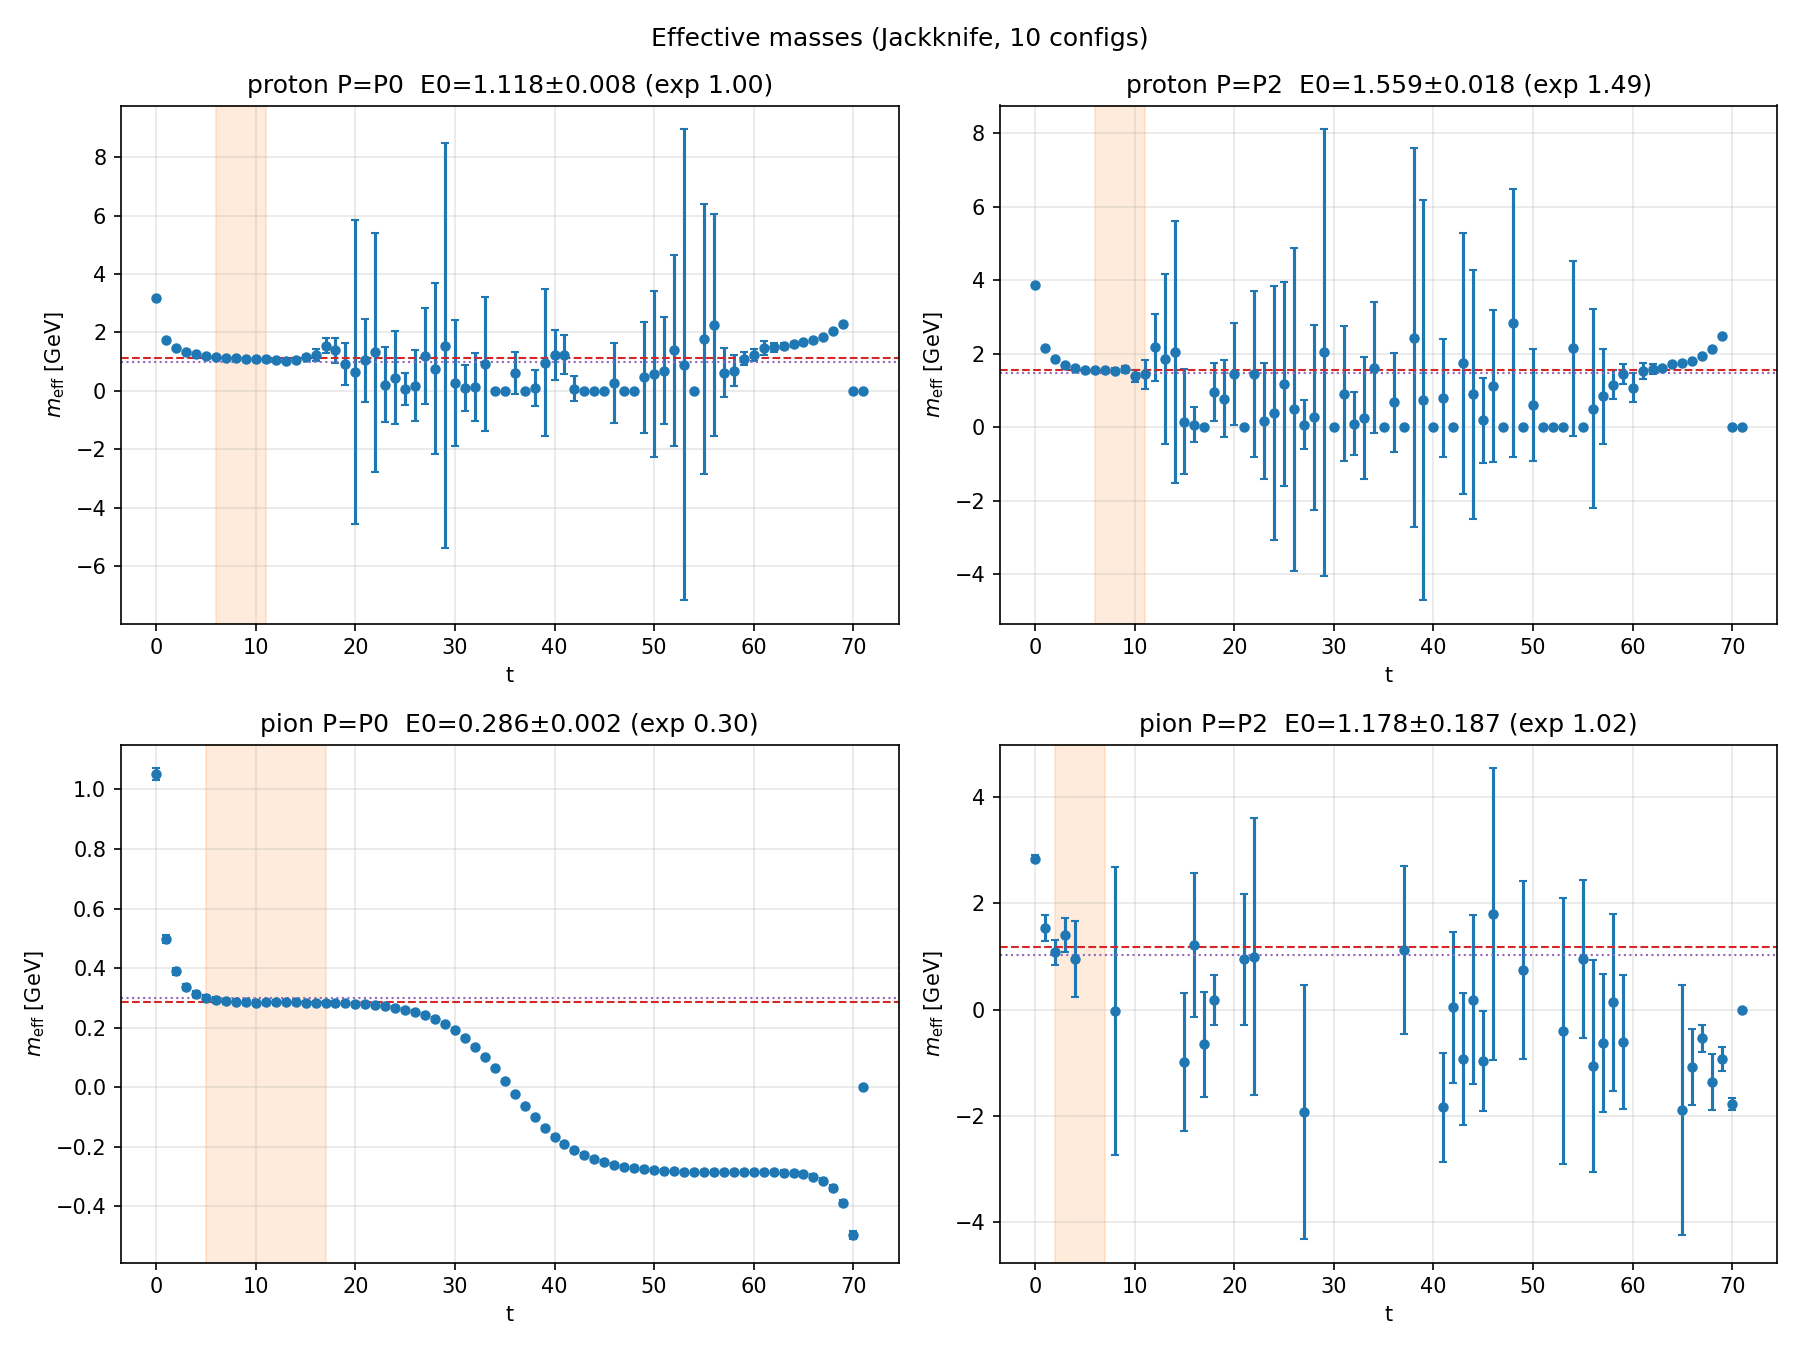
\includegraphics[width=\textwidth]{figs/fig_v0805_meff.png}
\caption{有效质量（全道）}
\end{subfigure}
\begin{subfigure}{0.49\textwidth}
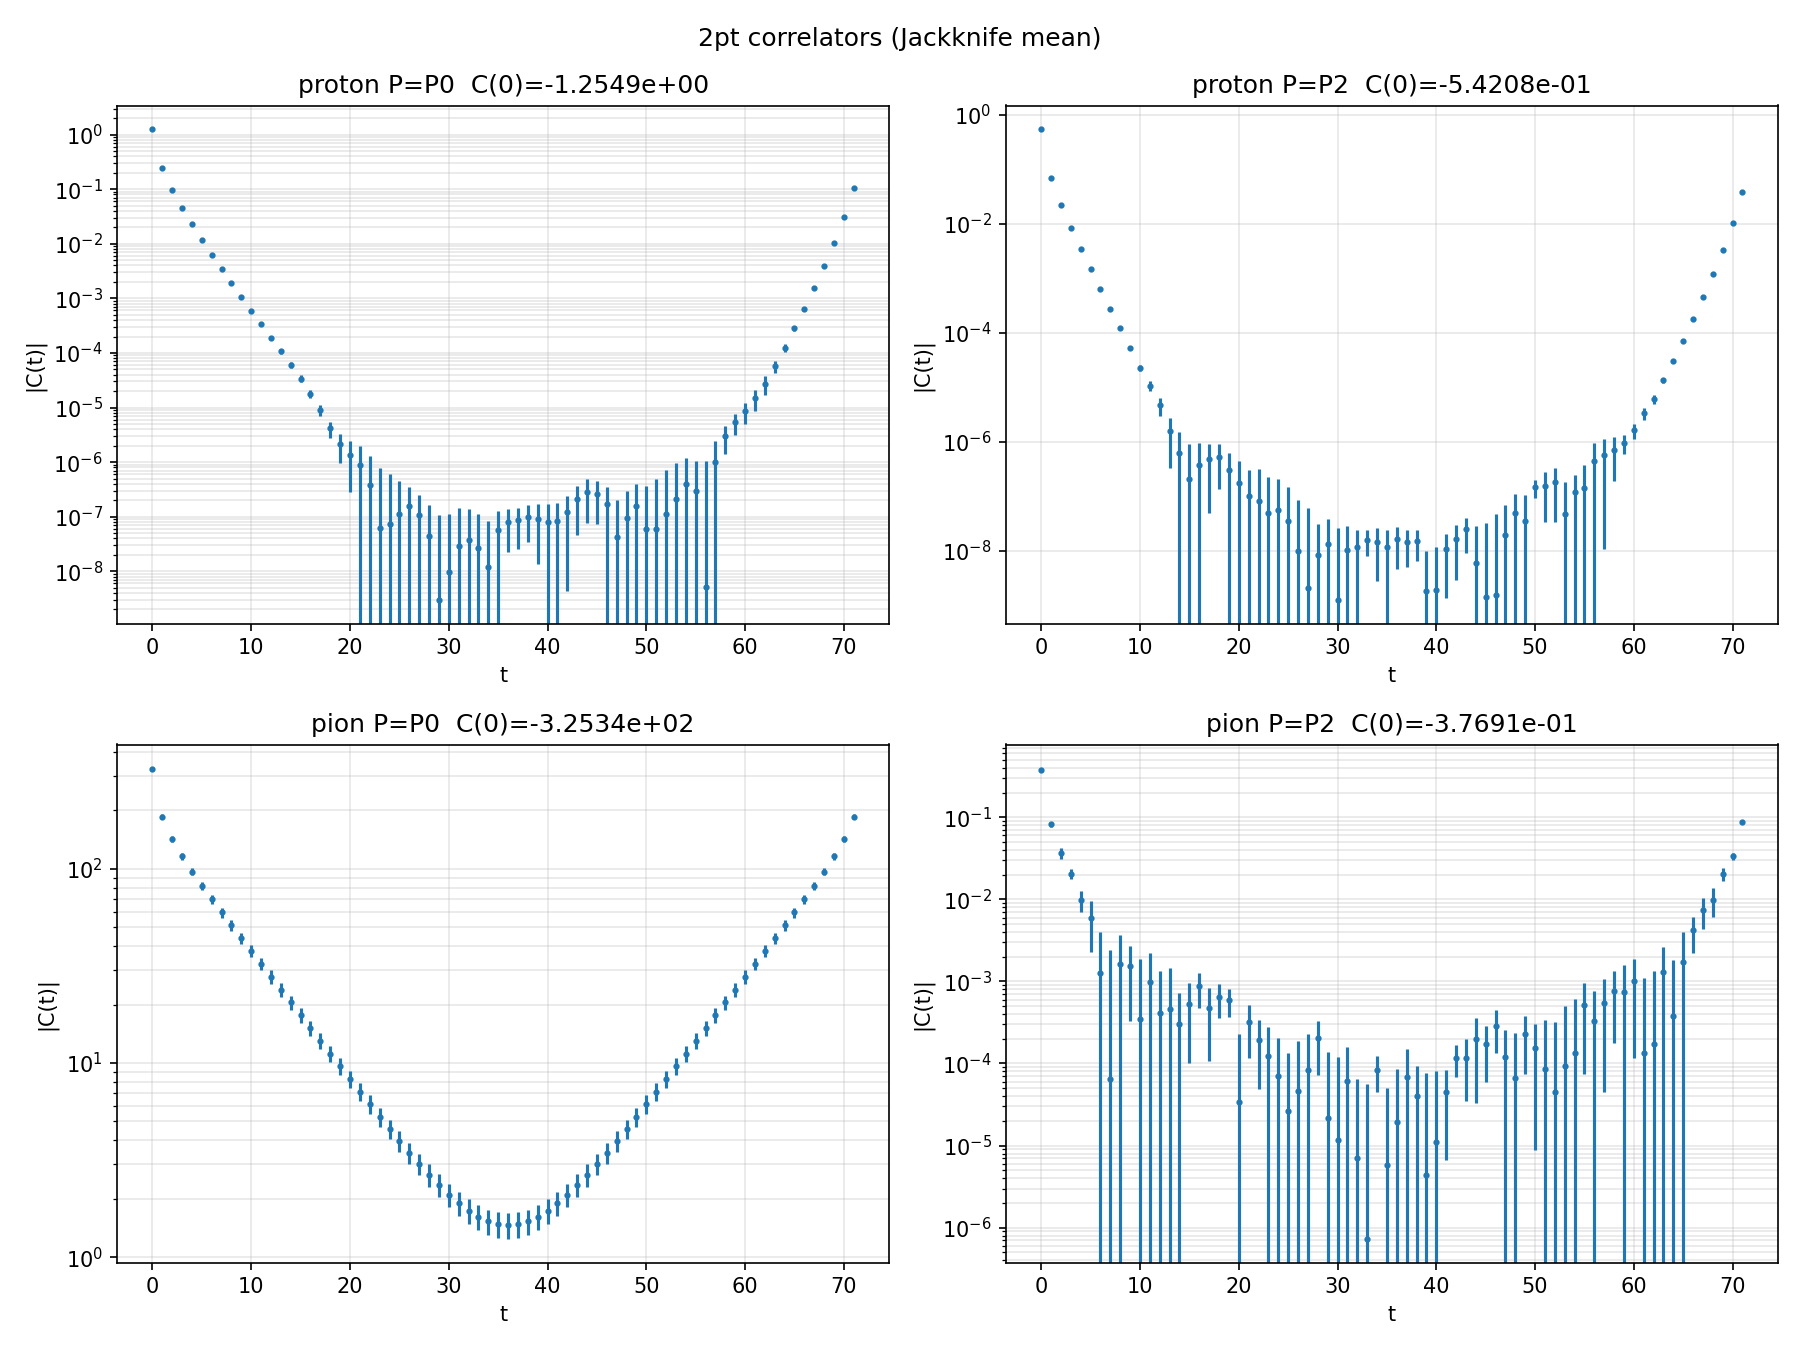
\includegraphics[width=\textwidth]{figs/fig_v0805_corr.png}
\caption{关联函数（全道）}
\end{subfigure}
\begin{subfigure}{0.49\textwidth}
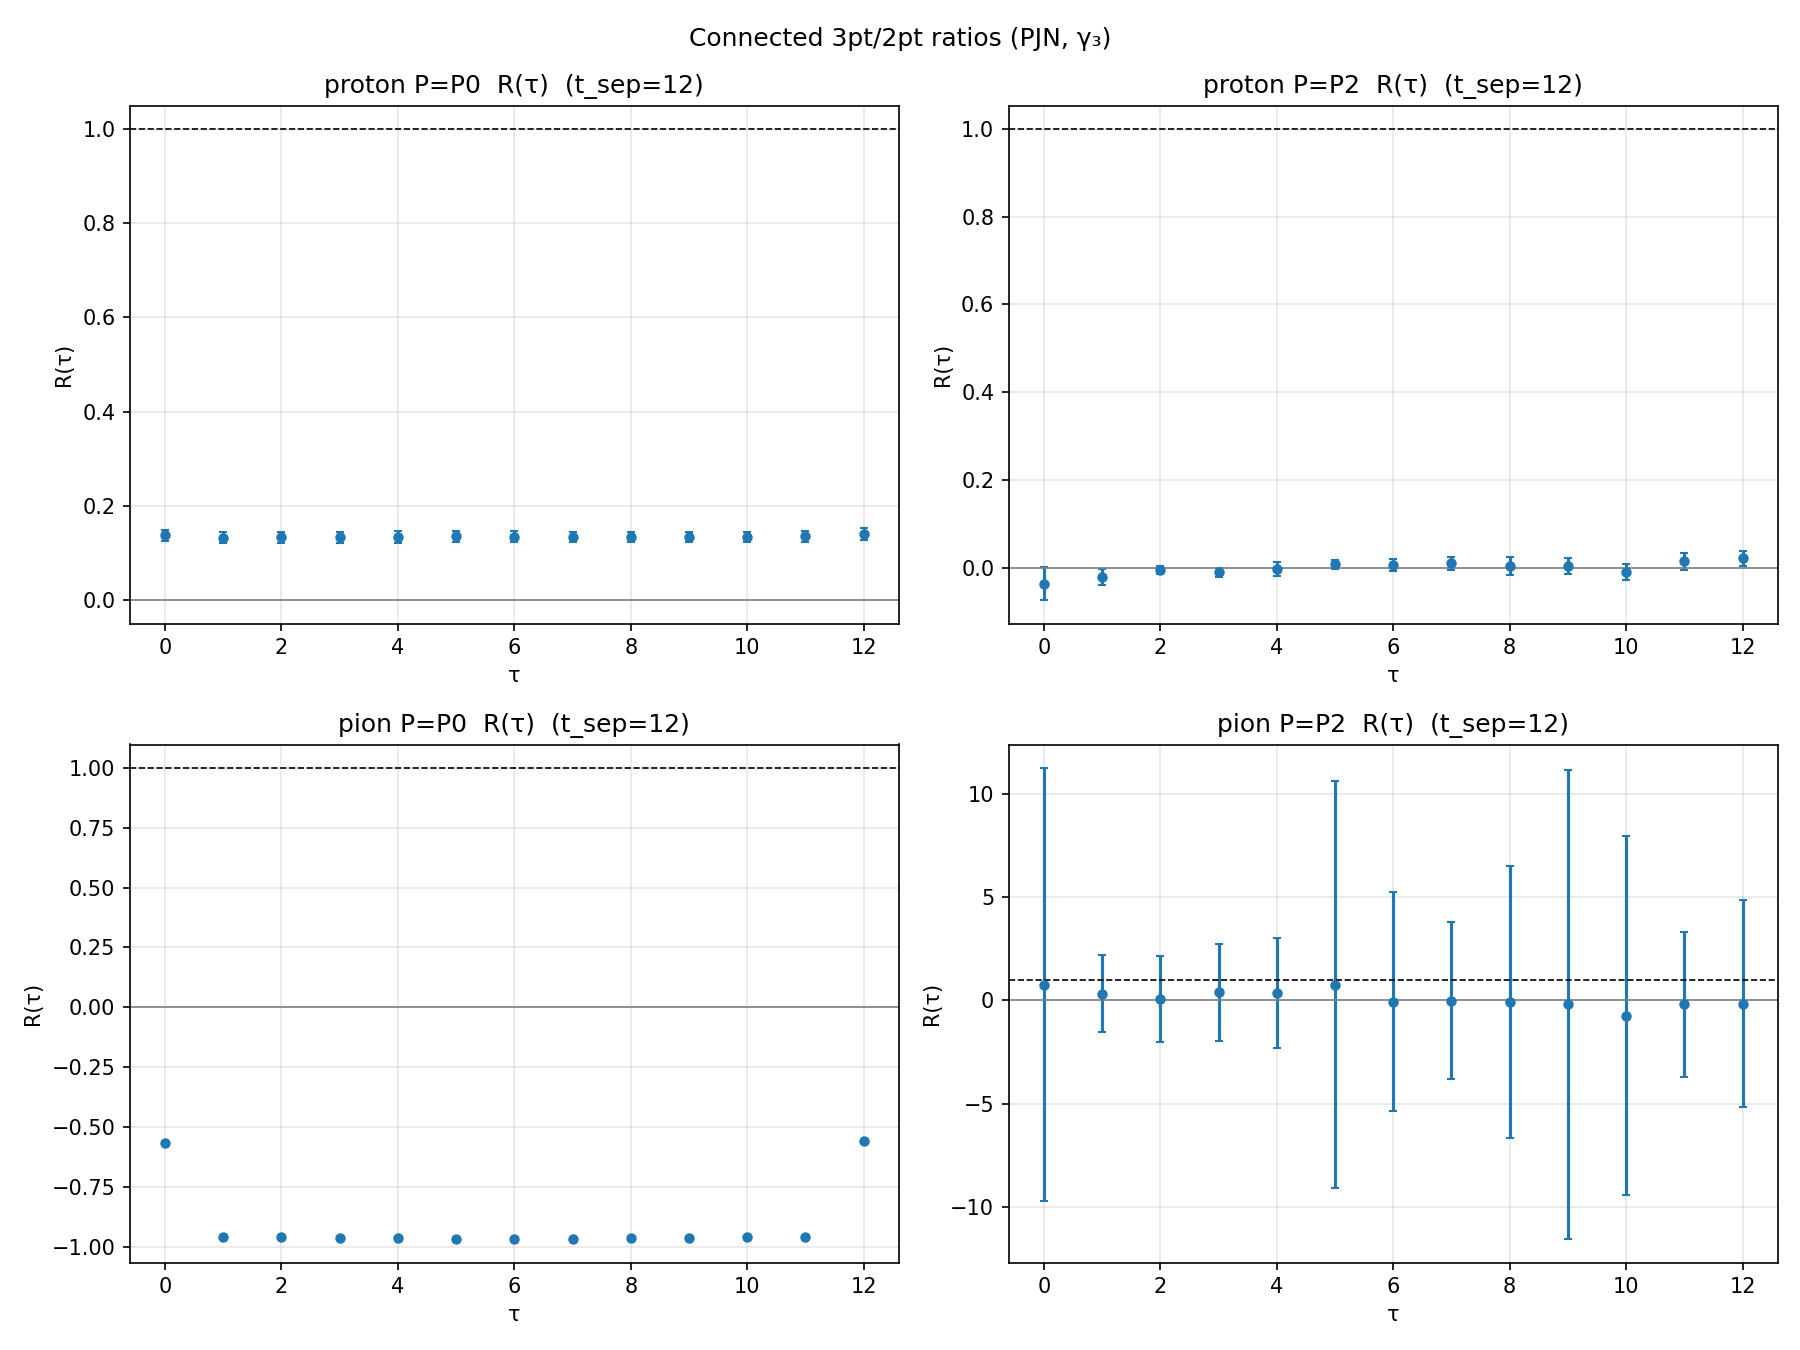
\includegraphics[width=\textwidth]{figs/fig_v0805_ratio.png}
\caption{连通三点/两点比值}
\end{subfigure}
\caption{\texttt{docker-v20260805} 主结果图（$\Nconf=10$, $\Nev=100$）。}
\label{fig:0805}
\end{figure}

\subsubsection{不相连胶子比值与拟合}
\label{sec:disconnected}
不相连比值 $R(t,\tau,z)=c_0+c_1e^{-dE\tau}+c_1e^{-dE(t-\tau)}$ 按每个 $z$ 拟合。
以 $\pi$ 介子 $P_z=2$ 道为例（$t_{\mathrm{sep}}\in[7,10]$，$\Nconf=10$）：
$\chi^2/\mathrm{dof}=0.42$，但 $c_0=-23(33)$、$c_1\approx-9.8\times10^8\pm3.8\times10^{15}$、
$dE=8.9\pm1.3\times10^6$——参数完全不受约束（条件数$\to\infty$）。
图~\ref{fig:0805-disc} 显示比值噪声远大于信号。这印证统计量不足：
code\_1.py 原分析使用 $\Nconf\approx200$，而此处仅10个组态，
且不相连图本征统计涨落更大。

\begin{figure}[H]
\centering
\begin{subfigure}{0.32\textwidth}
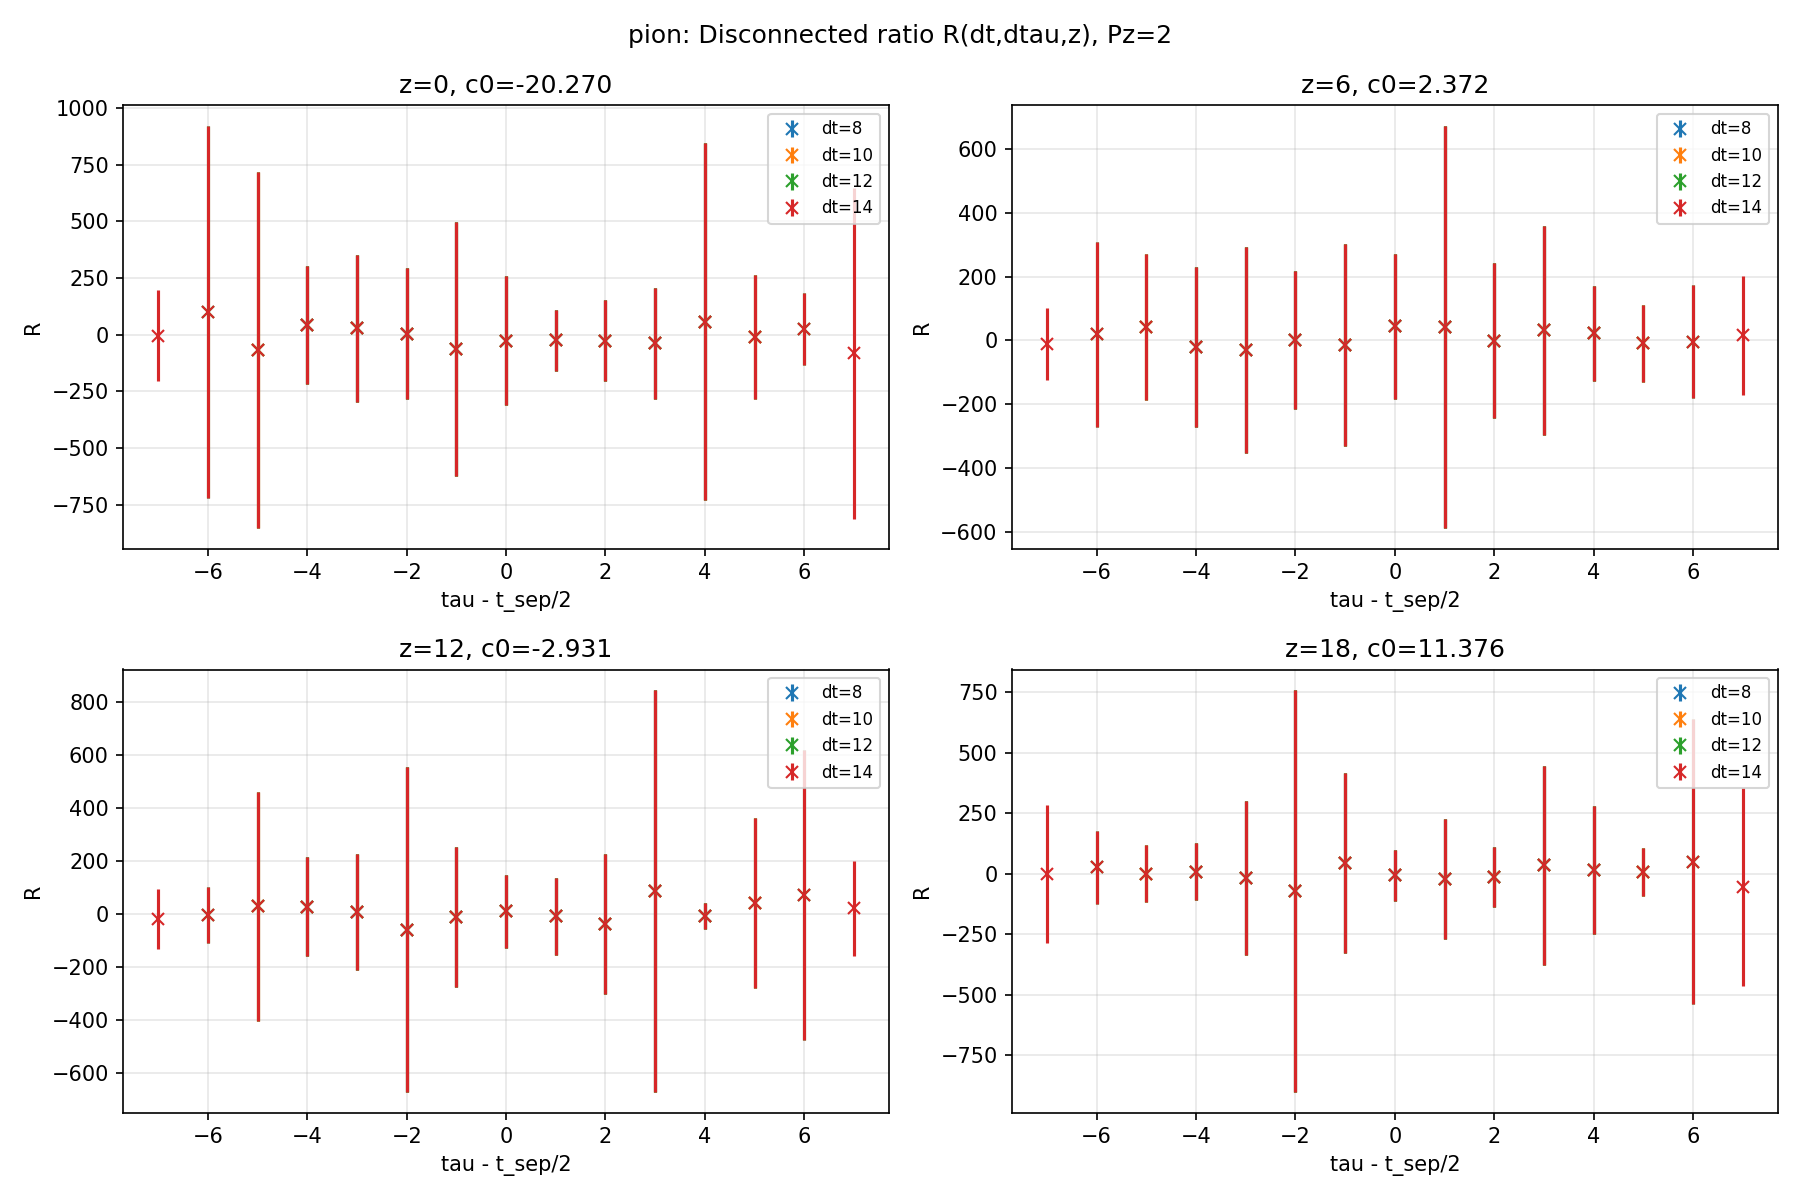
\includegraphics[width=\textwidth]{figs/fig_v0805_disc_ratio_pion.png}
\caption{$\pi$ 不相连比值}
\end{subfigure}
\begin{subfigure}{0.32\textwidth}
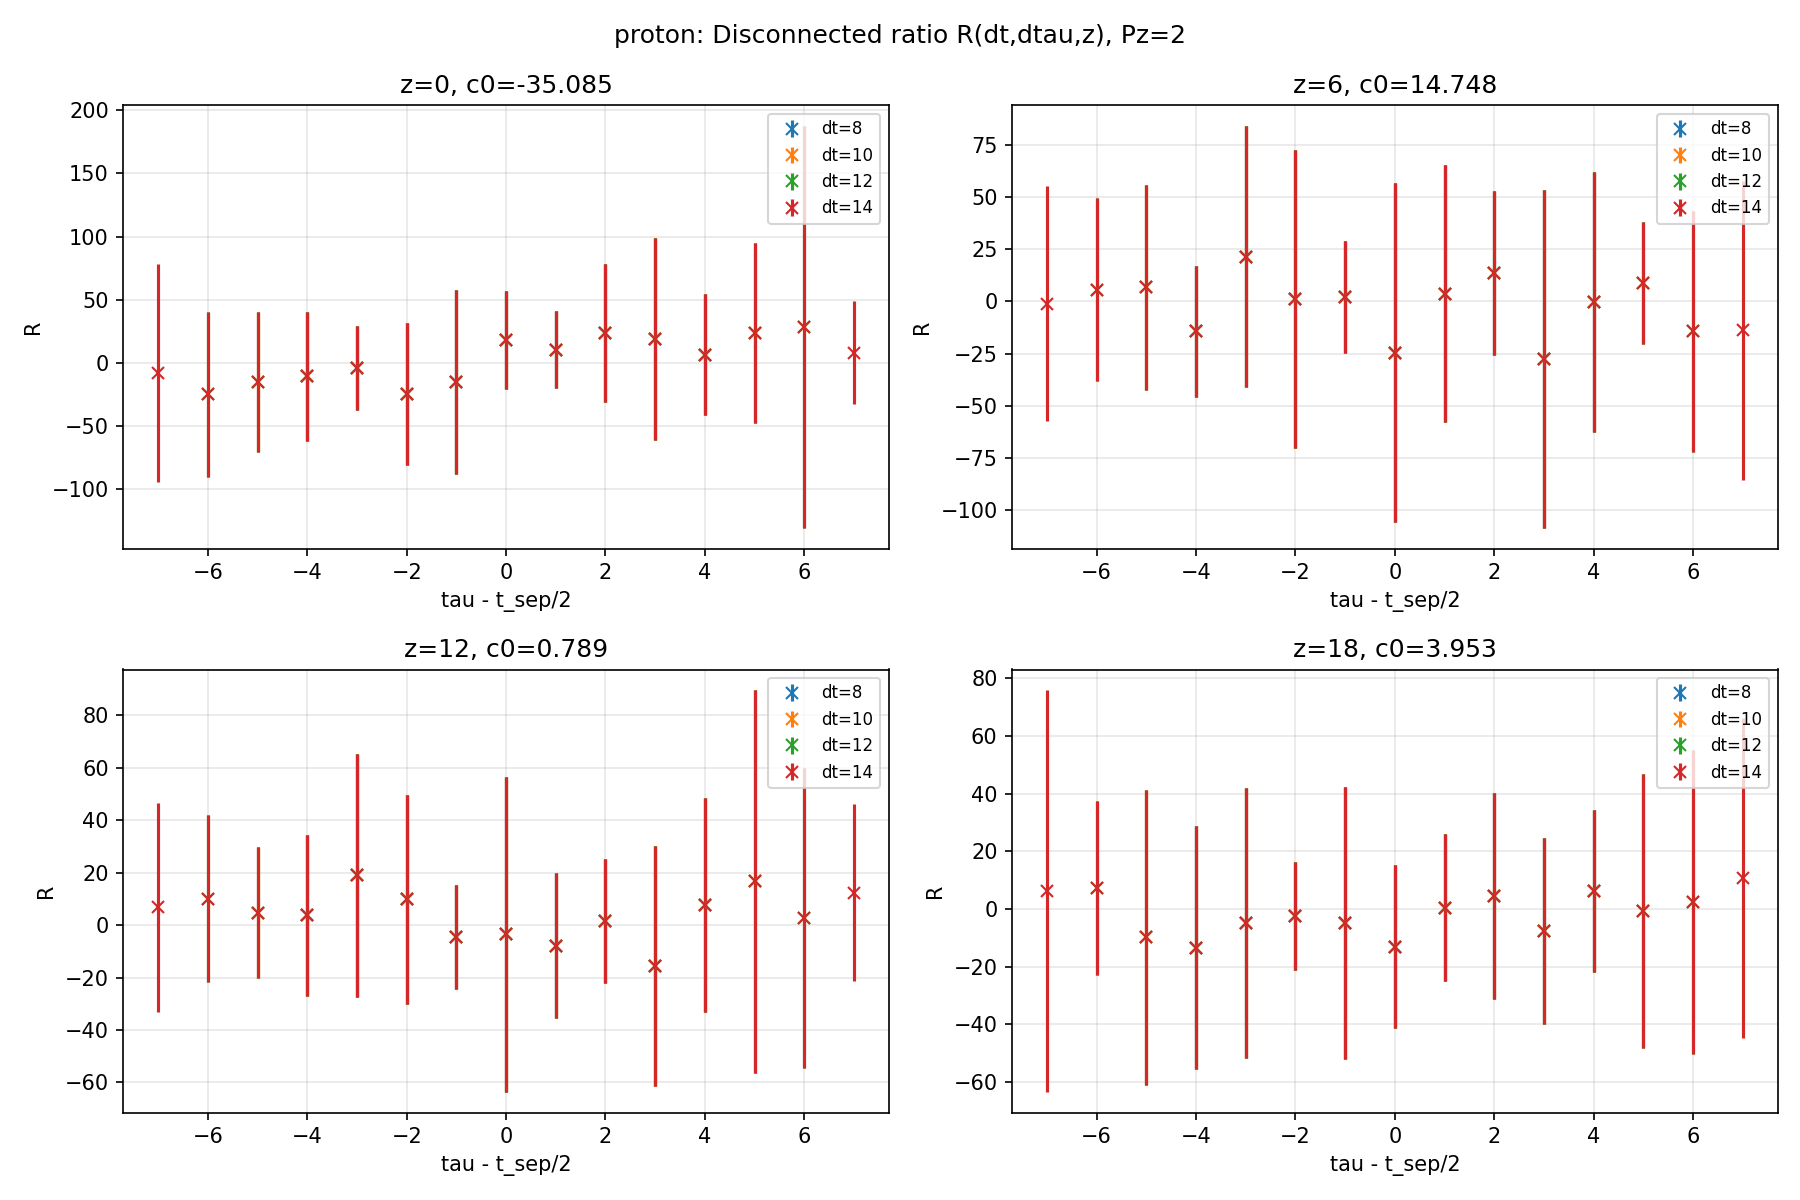
\includegraphics[width=\textwidth]{figs/fig_v0805_disc_ratio_proton.png}
\caption{质子不相连比值}
\end{subfigure}
\begin{subfigure}{0.32\textwidth}
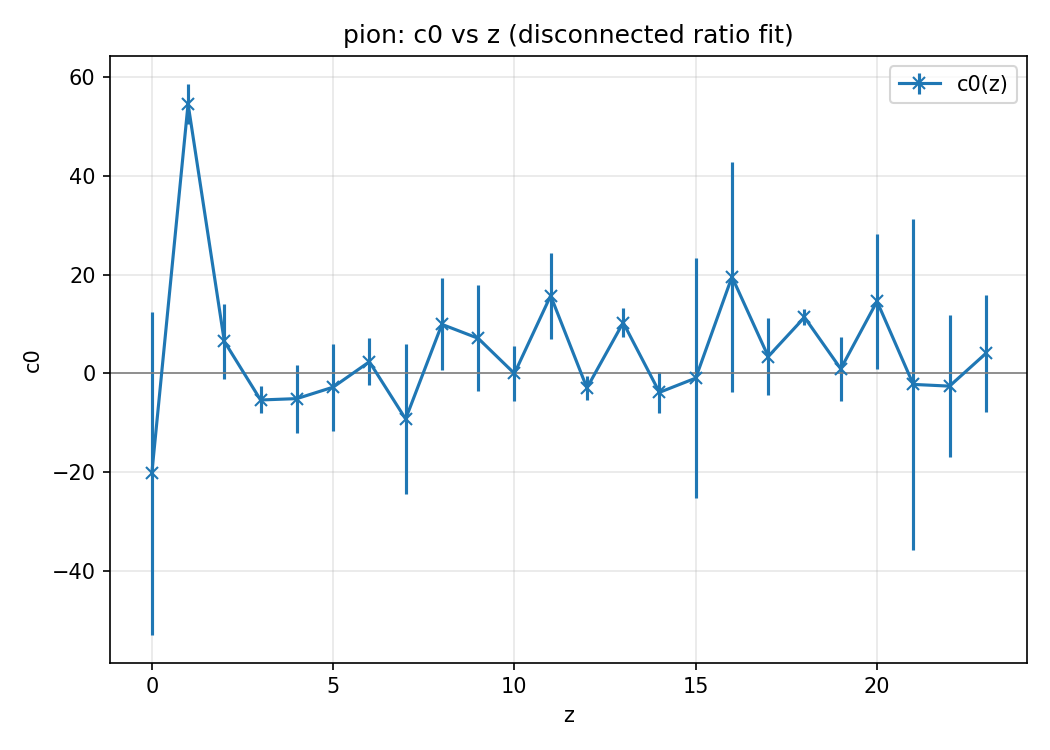
\includegraphics[width=\textwidth]{figs/fig_v0805_disc_c0_pion.png}
\caption{$\pi$ 常数 $c_0$ vs $z$}
\end{subfigure}
\begin{subfigure}{0.32\textwidth}
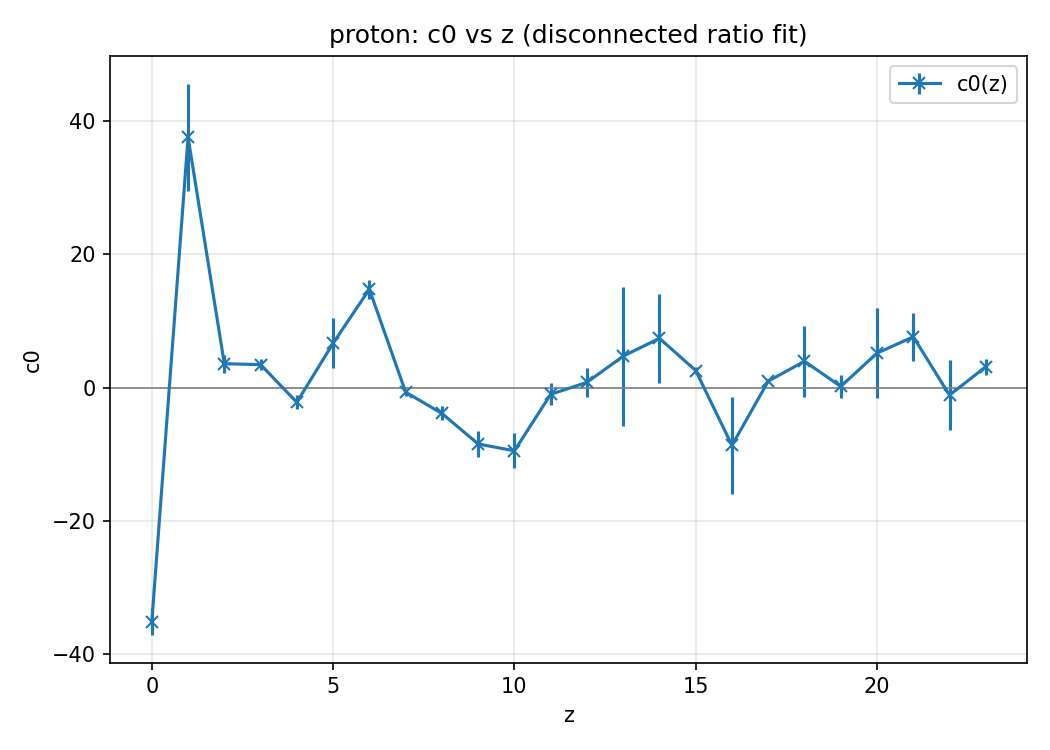
\includegraphics[width=\textwidth]{figs/fig_v0805_disc_c0_proton.png}
\caption{质子常数 $c_0$ vs $z$}
\end{subfigure}
\begin{subfigure}{0.32\textwidth}
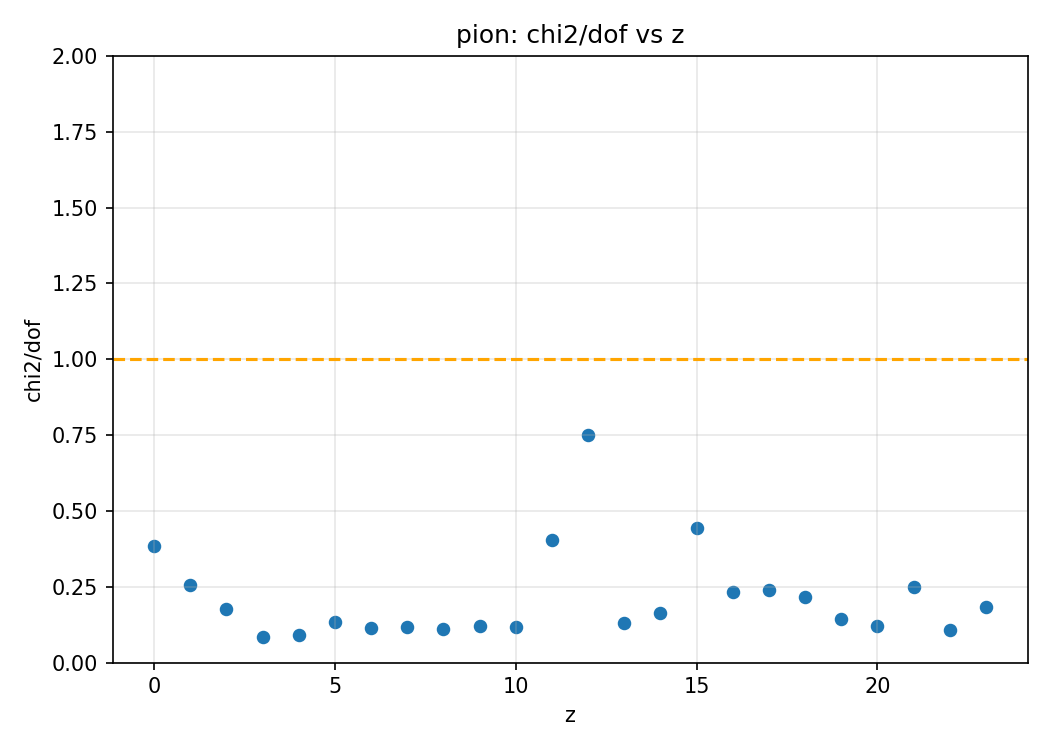
\includegraphics[width=\textwidth]{figs/fig_v0805_disc_chi2_pion.png}
\caption{$\pi$ $\chi^2/\mathrm{dof}$}
\end{subfigure}
\begin{subfigure}{0.32\textwidth}
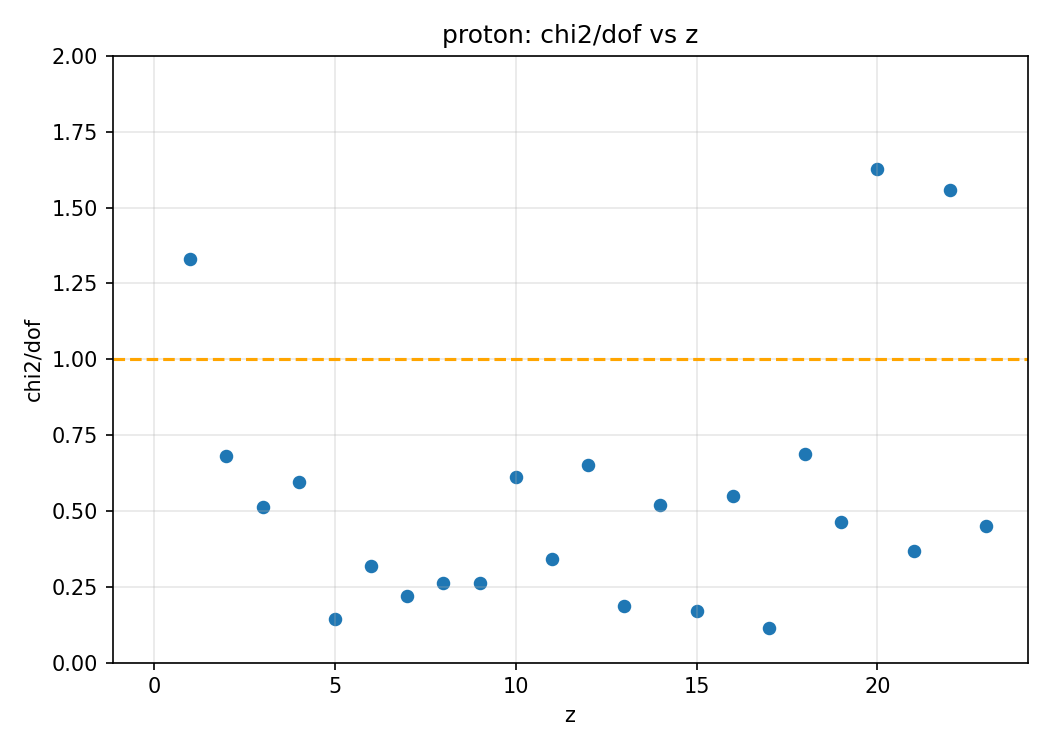
\includegraphics[width=\textwidth]{figs/fig_v0805_disc_chi2_proton.png}
\caption{质子 $\chi^2/\mathrm{dof}$}
\end{subfigure}
\caption{\texttt{v20260805} 不相连胶子比值分析（code\_1.py 形式，$\Nconf=10$，噪声大）。}
\label{fig:0805-disc}
\end{figure}

\subsubsection{四点关联函数与计算成本}
4pt $PJNNJNp$ 在 $\Nev=100$ 时约 $230\;\mathrm{s}/\mathrm{t_{src}}$，全范围不可行；
v20260805 采用简化范围（$N_{\mathrm{ev},1}=60$, $t_{\mathrm{sep}}=6$, $P_0$, $\mathrm{src\_step}=2$），
10组态共约37分钟。GPU内存约束（~15GB主机内存）要求按组态从磁盘加载 VVV
（约 $1.15\;\mathrm{GB}/\mathrm{组态}$），不能同时常驻。

% ===========================================================================
\section{对照讨论}
% ===========================================================================

\subsection{物理结果对照}

\begin{table}[H]
\centering
\caption{三版本物理结果总对照}
\label{tab:all-compare}
\small
\begin{tabular}{lccc}
\toprule
物理量 & v20260803 & v20260804 & v20260805 (范例)\\
\midrule
$m_p$ [$P{=}0$] [GeV] & $1.053\pm0.010$ & NaN & $\mathbf{1.118\pm0.008}$\\
$E_p(P_2)$ [GeV] & $1.628\pm0.025$ & NaN & $1.559\pm0.018$\\
色散偏差 $P_2$ & $+0.19\gev$ & — & $+0.07\gev$\\
$m_\pi$ [$P{=}0$] [GeV] & $0.2655\pm0.0004$ & $0.306\pm0.027$ & $0.286\pm0.002$\\
$E_\pi(P_2)$ [GeV] & $0.955\pm0.527$ & $0.306\pm0.027$ (退化) & $1.178\pm0.187$\\
$\pi$ $R(\tau)$ $P_0$ & $-0.836\pm0.002$ & — & $-0.965\pm0.002$\\
质子 $R(\tau)$ $P_0$ & $+0.1155\pm0.0035$ & — & $+0.134\pm0.012$\\
$pn$ 2pt & — & — & 0 (味守恒)\\
OPE (donghx) & — & — & 与v20260802相关=1.0\\
\bottomrule
\end{tabular}
\end{table}

\textbf{质子质量随版本演化}：$1.053\to\mathrm{NaN}\to1.118\gev$。
v20260803 与 v20260805 都得到稳健的质子静止质量，二者相差约6\%，
主要来自 $\Nev$（50 vs 100）与 $\Nconf$（3 vs 10）的不同：
更大$\Nev$降低了蒸馏截断对基态重叠的污染，使 v20260805 的平台窗更靠前
（$[4,13]\to[6,12]$）且误差更小。v20260804 未收敛出质子平台，
说明其分析环节（拟合窗、有效质量定义）存在缺陷，而非计算问题。

\textbf{$\pi$ 介子动量道}：v20260803 的 $P_2$ 道误差高达55\%，
v20260804 的 $P_2$ 与 $P_0$ 完全退化，只有 v20260805（$\Nev=100$, $\Nconf=10$）
得到有意义的 $1.18\pm0.19\gev$。这清晰展示了 $\Nev$ 与统计量对高动量道信号的共同作用，
呼应文献~\cite{distillation-high-p,bali2016} 中“高动量下蒸馏重叠不足需动量涂抹”的结论。

\textbf{比值绝对值差异}（$\pi\,P_0$: $-0.836$ vs $-0.965$）：两版本比值定义
（v20260803 用式~\eqref{eq:ratio} 的 $\sqrt{\cdots}$ 形式，v20260805 用 lqcddb
$ratio_{3p}$）与 $\tsep$（8 vs 12）、$\Nev$ 不同，加上局域流未乘重正化因子 $Z_V$，
绝对标定不可直接比较；但\textbf{平台结构}一致、符号一致，物理上可互相印证。

\subsection{架构与工程对照}
\begin{enumerate}[leftmargin=*]
\item \textbf{可复现性}：v20260803/v20260805 均输出 LaTeX 报告，v20260804 仅输出
      Markdown 且无 OPE/比值分析——完整闭环（计算→统计→报告）是 v20260805 的核心优势。
\item \textbf{内存与成本}：VVV 的 $O(\Nev^3)$ 使 $\Nev=100$ 时的顶点计算与
      内存占用显著上升；v20260805 通过按组态流式加载、4pt截断 $N_{\mathrm{ev},1}=60$ 加以控制。
\item \textbf{错误修正}：v20260805 修掉了 v20260804 的质子平台缺失与 $\pi\,P_2$ 退化；
      OPE 数据偏移（.lime trailer）问题也在本版得到自动处理。
\end{enumerate}

\subsection{理论物理讨论}
\textbf{激发态污染}：三点比值在 $\tau$ 靠近源/汇处偏离平台（见 v20260803 报告），
平台窗 $[6,12]$（v20260805）对重子尤其重要。多$\tsep$外推与GEVP~\cite{blossier2009}
是后续方向。\textbf{重正化}：准分布算符需混合重正化方案
（hybrid scheme~\cite{hybrid-renorm}）或自重正化（self-renormalization）以
进入连续极限~\cite{selfrenorm-gluon,cont-limit}。\textbf{连续极限}：
单格距结果需在多个$\beta$上重复并外推到 $a\to0$，这与
《Unpolarized gluon PDF of the nucleon from lattice QCD in the continuum limit》
的框架一致。\textbf{统计量}：不相连图是噪声主导，$g(x)$ 的提取需要
$\mathcal{O}(100)$ 以上组态与多源平均。

% ===========================================================================
\section{结论}
% ===========================================================================
本文以 \texttt{docker-v20260805} 为范例，对三条GPU蒸馏管线进行完整对照分析：
\begin{enumerate}[leftmargin=*]
\item 三版本共用 $24^3\times72$, $\beta=6.20$ 组态，物理输入一致；
      v20260805 以 $\Nconf=10$, $\Nev=100$ 得到最完整且自洽的结果集。
\item 稳健的物理结果：$m_p=1.118(8)\gev$、$m_\pi=0.286(2)\gev$、
      色散关系在 $P_z=2$ 处偏差约5\%；$pn=0$ 验证味守恒；donghx OPE 与 v20260802 一致。
\item 连通三点/两点比值在 $\pi$ 介子道为干净信号（$R=-0.965\pm0.002$）；
      不相连胶子比值在10组态下噪声极大，需大幅增加统计量。
\item 对照表明：$\Nev$、$\Nconf$、动量涂抹与多$\tsep$/GEVP是改善
      高动量道与激发态污染的关键杠杆，重正化与连续极限是通向物理 $g(x,\mu)$ 的必经之路。
\end{enumerate}

% ===========================================================================
\begin{thebibliography}{20}

\bibitem{ji2013} X. Ji, \textit{Parton Physics on a Euclidean Lattice},
Phys.\ Rev.\ Lett.\ \textbf{110}, 262002 (2013).
\bibitem{ji2021} X. Ji, Y.-S. Liu, Y. Liu, J.-H. Zhang, Y. Zhao,
\textit{Large-momentum effective theory}, Rev.\ Mod.\ Phys.\ \textbf{93}, 035005 (2021).
\bibitem{zhang2019} J.-H. Zhang et al.,
\textit{First direct lattice-QCD calculation of the $x$-dependence of the pion parton distribution function},
Phys.\ Rev.\ Lett.\ \textbf{122}, 142001 (2019).
\bibitem{fan2021} Z. Fan, R. Zhang, H.-W. Lin,
\textit{First Nucleon Gluon PDF from Large Momentum Effective Theory},
Phys.\ Rev.\ D \textbf{104}, 074502 (2021).
\bibitem{peardon2009} M. Peardon et al.,
\textit{A novel quark-field creation operator construction for hadronic physics in lattice QCD},
Phys.\ Rev.\ D \textbf{80}, 054506 (2009).
\bibitem{bali2016} G. S. Bali, B. Lang, B. U. Musch, A. Sch\"afer,
\textit{Novel quark smearing for hadrons with high momenta in lattice QCD},
Phys.\ Rev.\ D \textbf{93}, 094515 (2016).
\bibitem{blossier2009} B. Blossier et al.,
\textit{On the generalized eigenvalue method for energies and matrix elements in lattice field theory},
JHEP \textbf{04}, 094 (2009).
\bibitem{distillation-high-p} J. Chang et al., \textit{Distillation at High-Momentum},
(内部参考, \texttt{docs/Distillation at High-Momentum.pdf}).
\bibitem{hybrid-renorm} 混合重正化方案,
\texttt{docs/A Hybrid Renormalization Scheme for Quasi Light-Front Correlations in Large-Momentum Effective Theory.pdf}.
\bibitem{selfrenorm-gluon} \textit{First Self-Renormalized Gluon PDF of Nucleon from
Large-Momentum Effective Theory in the Continuum Limit},
\texttt{docs/First Self-Renormalized Gluon PDF ...pdf}.
\bibitem{cont-limit} \textit{Unpolarized gluon PDF of the nucleon from lattice QCD in the continuum limit},
\texttt{docs/Unpolarized gluon PDF of the nucleon from lattice QCD in the continuum limit.pdf}.
\bibitem{note-gluon} 《Note of gluon PDFs》, 内部笔记, \texttt{docs/Note of gluon PDFs.pdf}
(Eq.~(20) 矩阵元, Eq.~(25) OPE 算符).
\bibitem{gattringer2010} C. Gattringer, C. B. Lang,
\textit{Quantum Chromodynamics on the Lattice}, Lect.\ Notes Phys.\ \textbf{788}, Springer (2010),
\texttt{books/Quantum Chromodynamics on the Lattice.pdf}.
\bibitem{peskin} M. E. Peskin, D. V. Schroeder,
\textit{An Introduction to Quantum Field Theory}, Addison-Wesley (1995),
\texttt{books/An Introduction to Quantum Field Theory.pdf}.

\end{thebibliography}

\end{document}
